%Preamble
% noindent
\documentclass[12pt,a4paper]{article}       % Declares document size

\usepackage[
  margin=20mm,
  % paperwidth=21cm,
  % paperheight=170cm
]{geometry}          % Defines margins
\usepackage[utf8]{inputenc}                 % Defines encription
\usepackage[magyar]{babel}                  % Defines language
\usepackage{t1enc}                          % Correctly hyphenates vowels
\usepackage{type1cm, type1ec}

\usepackage{tikz}                           % Tikz and PGF for graphics
\usepackage{circuitikz}
\usetikzlibrary{intersections}
\usetikzlibrary{decorations.pathmorphing,patterns, patterns.meta}
\usetikzlibrary{decorations.text}
\usetikzlibrary{decorations.markings}
\usetikzlibrary{calc, arrows, angles, quotes}
\usepackage{pgf-pie}
\usepackage{qtree}
% \usepackage{pgfplots}
\usepackage{textgreek}
\usepackage{cancel}
\usepackage{caption}
\usepackage{subcaption}

\usepackage{xfrac}                          % Slanted fractions
\usepackage{lastpage}                       % Reference lastpage in footer
\usepackage{amsmath}                        % Math library
\usepackage{amssymb}                        % Symbols library
\usepackage{physics}                        % Physics library
\usepackage{subfiles}                       % Use subfiles
\usepackage{float}                          % Float
\usepackage{icomma}                         % Intelligent decimal separator
\usepackage{tabto}                          % Tab to a specific location in a document
\usepackage{multicol}                       % User nultiple cols
\usepackage{hyperref}                       % Mark refs
\usepackage[                                % More math font
  cal=rsfso, bb=ams
]{mathalpha}

\usepackage{fancyhdr}                       % Fancy design for pages
\renewcommand{\headrulewidth}{0.5pt}
\renewcommand{\footrulewidth}{0.5pt}
\setlength{\headheight}{20pt}
\pagestyle{fancy}
\cfoot{\thepage\ / \pageref{LastPage}}
\lhead{Polimertechnika felkészülést segítő kérdések}
\rhead{\emph{Készítette:} Sándor Tibor}

% \numberwithin{equation}{section}            % Numbering and indenting
% \numberwithin{figure}{section}
% \numberwithin{table}{section}
\setlength{\parindent}{0mm}
\setlength{\parskip}{.66em}

\usepackage{xparse}                         % Conditional commands
\usepackage{tcolorbox}                      % Colored boxes
\tcbuselibrary{breakable, skins, listings}
\newtcolorbox{cbox}[2]{
  shadow={0mm}{0mm}{-1.5mm}{fill=yellow!75!red,opacity=0.5},
  enhanced,
  float=htb,
  colback=red!5!white,
  colframe=red!75!black,
  title={#2},
}

\usepackage{chemfig}

\title{Polimertechnika felkészülést segítő kérdések \\ \large(BMEGEPTBM01) \\ \texttt{v1.4.0}}
\author{Sándor Tibor}

% indent

\newcounter{questionctr}
\newenvironment{question}[1]{
  \refstepcounter{questionctr}
  \begin{tcolorbox}[
    colback=gray!25,
    colbacktitle=red!10!yellow!50,
    enhanced,
    sharp corners,
    boxrule=0mm,
    frame hidden,
    breakable,
    enhanced jigsaw,
    title={\textcolor{black}{\textsc{\# \thequestionctr{} – #1}}}
  ]


}{\end{tcolorbox}}

\begin{document}

\maketitle
\thispagestyle{fancy}

\begin{question}{
    Mi a polimer; monomer; oligomer? Mi a polimerizáció és mi a degradáció? Mi
    a polimertechnika? Mi a műanyag?
  }
  A \textbf{monomer} polimerizációra alkalmas kisméretű molekula.
  \tcbline

  Az \textbf{ismétlődő egység} a kettős kovalens kötések felszakadása során jön
  létre.
  \tcbline

  Az ismétlődő egységek kovalens kötéssel összekapcsolódva makromolekulát, az
  ún. \textbf{polimermolekulát} hozzák létre. Ez a gyakorlatban több száz,
  általában ezer ismétlődő egység összekapcsolását jelenti.
  \tcbline

  Az \textbf{oligomer} a polimerhez hasonló, de alapvetően kisebb tömegű
  molekula. Polimerizációs foka a tizes nagyságrendbe esik. A polimerekkel
  ellentétben itt pár ismétlődő egység hozzáadása vagy elvétele jelentősen
  befolyásolja a molekula tulajdonságait.
  \tcbline

  A polimereket \textbf{polimerizáció} révén alakítjuk ki. Történhet folyamatos
  (láncrealció) és lépcsős (polikondenzáció, poliaddíció) módon is. A
  polimerizációval ellentétes folyamat a \textbf{degradáció}, amely során a
  polimer láncmolekulák statisztikusan töredeznek, vagy a végük rövidül (más
  néven depolimerizáció), illetve csoportok válnak le a polimer láncról
  (elimináció).
  \tcbline

  A \textbf{polimertechnika} minden olyan műszaki tevékenység, amit
  polimerekkel végzünk. (előállítás, anyagtudomány, vizsgálat, módosítás,
  feldolgozás, műszaki feladatok)
  \tcbline

  A \textbf{műanyagok} részben vagy egészben mesterségesen előállított
  polimerek. Tágabb értelemben a polimerek adalékolt változata is műanyag.
\end{question}


\begin{question}{
    Mit jelent a polimerizációs fok és mi a szerepe? Mi a különbség a monomer
    és az ismétlődő egység között? Mutassa be a tömegpolimerek ismétlődő
    egységét és magyarázza el, hogy milyen anyagtulajdonságokra
    következtethetünk ebből.
  }
  A polimerizációs fok (\textbf{DP}, \emph{degree of polymerization}) azt
  fejezi ki, hogy hány monomerből polimerizáltuk az adott molekulaláncot.
  Polimerizáció során a monomerek ismétlődő egységekké alakulnak. A kettős
  kötések felbomlanak.
  \tcbline

  % noindent
  % PE
  \underline{\textbf{\textit{Polietilén:}}} \\
  A polietilén ún. \textbf{poliolefin} (Ismétlődő egységébe csak szénből és
    hidrogénből áll). Monomerje az \textbf{etilén}, melyet kőolaj pirolízise
  során állítanak elő. \textbf{Polimerizációs láncreakcióval} állítják elő.
  \textbf{Részben kristályos, hőre lágyuló, apoláros} polimer. Opálos, szívós
  anyag, kis merevséggel és sűrűséggel rendelkezik. Nehéz oldatba vinni.
  \textbf{Hidrofób}, \textbf{szigetelő}, de nem aromazáró.
  \begin{figure}[H]
    \centering

    \setchemfig{
        atom sep=2em,
        bond style={line width=1pt,red}
    }
    \schemestart
    $n \; \cross$
    \chemfig{C(-[6]H)(-[2]H)=C(-[6]H)(-[2]H)}
    \arrow(.mid east--.mid west)
    \chemfig{
      \vphantom{X}
      -[@{op}]C(-[2]H)(-[6]H)
      -C(-[@{cp}])(-[2]H)(-[6]H)
      -\vphantom{X}
    }
    \polymerdelim[
      delimiters ={[]},
      height = 2.25em,
      depth = 2.75em,
      indice = n
    ]{op}{cp}
    \schemestop \chemnameinit{}

    \caption{Polietilén előállítása}
  \end{figure}
  \textbf{Feldolgozása:}
  \\
  Fröccsöntéssel, extrúzióval, extrúziós fúvással, rotációs öntéssel.
  Nenehezen ragasztható, hegeszteni, címkézni érdemes.
  \\[2mm]
  \textbf{Fajtái:}
  \begin{itemize}
    \item LDPE – sok hosszú elágazás, kis kristályos részarány
    \item HDPE – sokkal kevesebb, rövid elágazás, nagyobb kristályos részarány
    \item LLDPE – nagyon sűrűn nagyon sok elágazás, kevés áthurkolódás
    \item UHMWPE – nagy szívósság, kis molekulasűrűség
  \end{itemize}
  \textbf{Felhasználása:}
  \\
  Csomagolófóliák, zacskók, mezőgazdasági fóliák, kábelszigetlések, kültéri
  székek (HDPE), csípőprotézisek (UHMWPE), gépelemek (UHMWPE)
  \tcbline
  

  % PP
  \underline{\textbf{\textit{Polipropilén:}}} \\
  A polipropilén szintén \textbf{poliolefin} anyag, Monomerje a
  \textbf{propilén}, belőle láncreakcióval állítják elő a PE-t. \textbf{Részben
    kristályos, hőre lágyuló}, erősen \textbf{apoláros} molekula. Sűrűsége
  nagyon kicsi ($0,9 \, \mathrm{\sfrac{g}{cm^3}}$). Jó \textbf{ütésálló}, nagy
  energia-elnyelő képessége van. Rossz UV állósága miatt sárgulásra hajlamos.
  Hidegállóképessége sem az igazi, gyakran társítják \textbf{erősítőanyagokkal}
  (farost, üvegszál). Vegyileg ellenálló, jó \textbf{szigetelő}.
  \begin{figure}[H]
    \centering
    
    \setchemfig{
        atom sep=2em,
        bond style={line width=1pt,red}
    }
    \schemestart
    $n \; \cross$
    \chemfig[angle increment=60]{
      C(-[2]H)(-[4]H)
      =C(-[1]H)
      -[5]C(-[4]H)(-[5]H)(-[6]H)
    }
    \arrow(.mid east--.mid west)
    \chemfig{
      \vphantom{X}
      -[@{op,.25}, 1.25]C(-[::+120]H)(-[::+240]H)
      -C(-[::+60]H)(-[6]C(-[6]H)(-[::-60]H)(-[::+60]H))
      -[@{cp,.875},1.5]\vphantom{X}}
    \polymerdelim[
      delimiters ={[]},
      height = 2.25em,
      depth = 4.75em,
      indice = n
    ]{op}{cp}
    \schemestop \chemnameinit{}

    \caption{Polipropilén előállítása}
  \end{figure}
  \textbf{Feldolgozása:}
  \\
  PE-hez hasonló technológiákkal: fröccsöntés, extrúzió.
  \\[2mm]
  \textbf{Felhasználása:}
  \\
  Műszálak, kötözőzsinórok, zsákok, hevederek, cserepek, orvosi eszközök,
  lökhárító (EPDM gumi – etilén és dién hozzáadásával).
  \tcbline
  
  
  % PVC
  \underline{\textbf{\textit{Polivinil-klorid:}}} \\
  A PVC \textbf{amorf, hőre lágyuló} polimer, vinil-kloridból állítják elő
  \textbf{polimerizációs láncreakcióval}. Klór atomok \textbf{ataktikusan}
  helyezkednek el, molekulákon hosszú \textbf{elágazások találhatók} (mint
    LDPE). Oda kell figyelni a feldolgozása során, ugyanis \textbf{hőbomlásakor
    sósav} keletkezik, viszont önmagában inert és  ártalmatlan. Feldolgozása
  során \textbf{adalékolják}, \textbf{lágyítókat} adnak hozzá, melyek
  egészségre ártalmasak lehetnek. (Lágyítók a molekulák közötti másodrendű
  kötések mennyiségét csökkentik.) Rengetek más adalékot is fel tud venni:
  kvarchomok, talkum, farost.
  \begin{figure}[H]
    \centering

    \setchemfig{
        atom sep=2em,
        bond style={line width=1pt,red}
    }
    \schemestart
    $n \; \cross$
    \chemfig{C(-[6]H)(-[2]H)=C(-[6]Cl)(-[2]H)}
    \arrow(.mid east--.mid west)
    \chemfig[
      atom sep=2em,
      bond style={line width=1pt,red}
    ]{\vphantom{X}-[@{op}]C(-[2]H)(-[6]H)-C(-[@{cp}])(-[2]H)(-[6]Cl)-\vphantom{X}}
    \polymerdelim[
      delimiters ={[]},
      height = 2.25em,
      depth = 2.75em,
      indice = n
    ]{op}{cp} 
    \schemestop \chemnameinit{}
    
    \caption{Polivinil-klorid előállítása}
  \end{figure}
  \textbf{Feldolgozása:}
  \\
  Extrúzió, extrúziós fúvás, kalanderezés, bevonatolás, fröccsöntés
  \\[2mm]
  \textbf{Felhasználása:}
  \\
  Csövek, ablak- és ajtókeretek, kábelek bevonatai, gumicsizma, linóleum,
  fogantyúk, úszógumi.
  \tcbline
  

  % PET
  \underline{\textbf{\textit{Polietilén-tereftalát:}}} \\
  A PET egy \textbf{részben kristályos, hőre lágyuló} polimer, a telített
  \textbf{poliészterek} családjába tartozik. Előállítása
  \textbf{polikondenzációval} történik etilén-glikolból és tereftálsavból.
  Kristályosodása a hűtés sebességével befolyásolható, minél gyorsabban hűtjük,
  annál kisebb kristályos részarányt kapunk. \textbf{Műszaki polimer}, jó
  mechanikai tulajdonságokkal rendelkezik. Jó víz- és gázzáró képességű, UV
  stabil, szigetelő, viszont ha nincsen kiszárítva, akkor hidrolízissel
  degradálódik.
  \begin{figure}[H]
    \centering

    \setchemfig{
        atom sep=2em,
        bond style={line width=1pt,red},
        arrow angle=-90,
    }
    \schemestart
    $n \; \cross$
    \chemname{\chemfig[angle increment=60]{
      C(-[2]HO)(=[4]O)
      -*6([,.75]-=-(-C(-[1,1]OH)(=[5,1]O))=-=)
    }}{Tereftálsav}
    \+
    $n \; \cross$
    \chemname{\chemfig{HO-CH_2-CH_2-OH}}{Etilén-glikol}
    \arrow
    \chemfig[
      atom sep=2em,
      bond style={line width=1pt,red}
    ]{
      \vphantom{X}
      -[@{op,0.25}, 1.25]C(-[::+120]H)(-[::+240]H)
      -C(-[::+60]H)(-[::-60]H)
      -O
      -[::-60]C(=[::-60]O)
      -*6([,.75]-=-([,1]-C(=[::-60]O)-[::+60]O(-[@{cp}])-\vphantom{X})=-=)
    }
    \+
    $2n \; \cross$
    \chemfig{H_2O}
    \polymerdelim[
      delimiters ={[]},
      height = 2.5em,
      depth = 4.5em,
      indice = n
    ]{op}{cp}
    \schemestop \chemnameinit{}

    \caption{Polietilén-tereftalát előállítása}
  \end{figure}
  \textbf{Feldolgozása:}
  \\
  Fröccsfúvással, illetve fóliagyártási eljárásokkal, melegalakítással.
  Újrahasznosítótt PET-ből extrudált műszálat (PES) készítenek.
  \\[2mm]
  \textbf{Felhasználása:}
  \\
  Palackok, műszálak (PES), csomagolás.
  \tcbline


  % PS
  \underline{\textbf{\textit{Polisztirol:}}} \\
  A poisztirol egy jellemzően \textbf{amorf} szerkezetű, \textbf{apoláros},
  \textbf{aromás} polimer. Sztirol polimerizációs \textbf{láncreakciójával}
  állítják elő. Könnyen színezhető, \textbf{szag-} és \textbf{ízmentessé}
  tehető, ezért egyszerhasználatos élelmiszeripari termékek alapanyaga. Nagy
  modulusú, ennélfogva rideg, törékeny, rossz UV-álló. Nedvességet nem vesz
  fel, termikus degradációra sem hajlamos. Festhető, címkézhető, anyagában
  színezhető.
  \begin{figure}[H]
    \centering
    
    \setchemfig{
        atom sep=2em,
        bond style={line width=1pt,red}
    }
    \schemestart
    $n \; \cross$
    \chemfig[angle increment=60]{
      C(-[4]H)(-[2]H)
      =C(-[1]H)(-[5]*6([5, .75]-=-=-=))
    }
    \arrow(.mid east--.mid west)
     \chemfig[
      atom sep=2em,
      bond style={line width=1pt,red}
    ]{
      \vphantom{X}
      -[@{op,.25}, 1.25]C(-[::+120]H)(-[::+240]H)
      -C(-[@{cp,.75}, 1.25])(-[::+60]H)(-[6]*6([6,.75]-=-=-=))
      -\vphantom{X}
    }
    \polymerdelim[
      delimiters ={[]},
      height = 2.25em,
      depth = 5.5em,
      indice = n
    ]{op}{cp}
    \schemestop \chemnameinit{}

    \caption{Polisztirol előállítása}
  \end{figure}
  \textbf{Feldolgozása:}
  \\
  Melegalakítással, extrúzióval, expandálással, akár fröccsöntéssel.
  \\[2mm]
  \textbf{Felhasználása:}
  \\
  Műanyag evőeszközök és tányérok, játékok, poharak, pipetták,
  gyógyszertárolók. CD-tartó (HiPS), EPS (expandált), XPS (extrudált) habok
  szigetelésre.
% indent
\end{question}


\begin{question}{
    Csoportosítsa a polimer szerkezeti anyagokat (lineáris, térhálós stb.).
    Vázolja fel és magyarázza el az egyes mesterséges polimer típusok
    jellegzetes szerkezetét. Az anyagszerkezettani különbség milyen
    különbségekhez vezet az anyagtulajdonságokban?
  }
  \Tree[.{Polimerek}
      {Természetes}
      [.{Mesterséges}
          [.{Lineáris}
              {Részben\\kristályos}
              {Amorf}
          ]
          [.{Térhálós}
              {Ritkán\\térhálós}
              {Sűrűn\\térhálós}
          ]
      ]
  ]
  \tcbline

  \underline{\textbf{\textit{Lineáris polimerek:}}} \\
  A lineáris polimerek viselkedésük szerint \textbf{hőre lágyulóak}.
  Feldolgozásukkor folyékony halmazállapotba hozhatóak, majd hűtéssel újra
  megszilárdíthatóak. A folyamat \textbf{reverzibilis}. Emiatt
  \textbf{termoplasztikus} anyagoknak is szokás nevezni őket. Szerkezetükben
  lineárisak, de lehetnek a molekulákon \textbf{elágazások}, viszont a
  molekulák között csak \textbf{fizikai} kötések alakulnak ki, kémiaiak nem.
  Ezért a molekulák egymáshoz képest elcsúszhatnak. A lineáris polimerek
  lehetnek:
  \begin{itemize}
    \item Részben kristályos polimerek:
          PET, PE, PP, PA, PTFE
    \item Lineárisan amorf anyagok:
          PVC, PS, ABS, PC, PMMA, SAN
  \end{itemize}
  \tcbline

  \underline{\textbf{\textit{Térhálós polimerek:}}} \\
  A térhálós polimerek viselkedésük szerint \textbf{hőre keményedőek}.
  Ezek az anyagok csak \textbf{amorfak} lehetnek. A molekulák között
  \textbf{kémiai} és \textbf{fizikai} kötések is kialakulnak, ezért nem
  ömleszhetőek meg, ezért a polimerizációt közvetlenül a termék gyártása előtt
  kell elvégezni (irreverzibilis). A térhálós polimerek lehetnek:
  \begin{itemize}
    \item Ritkán térhálós elasztomerek: NR, SBR, NBR
    \item Sűrűn térhálós duromerek (műgyanták): EP, UP, VE
  \end{itemize}
\end{question}


\begin{question}{
    Miért szén-alapú a polimerek többsége? A szénnek milyen allotróp
    módosulatait ismeri?
  }
  A polimerek lehetnek:

  \begin{multicols}{3}
    \centering
    \chemfig[
    atom sep=2em,
    bond style={line width=1pt,red}
    ]{\phantom{X}
    -C(-[2]\vphantom{X})(-[6]\vphantom{X})
    -C(-[2]\vphantom{X})(-[6]\vphantom{X})
    -C(-[2]\vphantom{X})(-[6]\vphantom{X})
    -\phantom{X}}
    \\[2mm]
    Homogén\\szénvázú\\szerves

    \chemfig[
    atom sep=2em,
    bond style={line width=1pt,red}
    ]{\phantom{X}
    -C(-[2]\vphantom{X})(-[6]\vphantom{X})
    -X
    -C(-[2]\vphantom{X})(-[6]\vphantom{X})
    -\phantom{X}}
    \\[2mm]
    Heterogén\\szénvázú\\szerves

    \chemfig[
    atom sep=2em,
    bond style={line width=1pt,red}
    ]{\phantom{X}
    -Si(-[2]\vphantom{X})(-[6]\vphantom{X})
    -O
    -Si(-[2]\vphantom{X})(-[6]\vphantom{X})
    -\phantom{X}}
    \\[2mm]
    Heterogén\\szilíciumvázas\\szervetlen
  \end{multicols}
  \tcbline
  \begin{center}
    \chemfig{C} \quad $6p^+ \;\; 6n^0 \;\; 6e^-$
  \end{center}
  Az emberi élet is szén alapú. 4 másik atommal tud kovalens kötést létesíteni.
  $109,5^\circ$-os kötésszög jellemzi (\chemfig{CH_4}). \textbf{Allotróp
    módosulatai}:
  \begin{multicols}{5}
    \begin{itemize}
      \item gyémánt,
      \item grafit,
      \item fullerén,
      \item amorf C,
      \item grafén.
    \end{itemize}
  \end{multicols}

  \begin{figure}[H]
    \centering
    \definesubmol\fragment1{
    (-[:#1,0.85,,,draw=none] -[::126]-[::-54](=_#(2pt,2pt)[::180])
    -[::-70](-[::-56.2,1.07]=^#(2pt,2pt)[::180,1.07])
    -[::110,0.6](-[::-148,0.60](=^[::180,0.35])-[::-18,1.1])
    -[::50,1.1](-[::18,0.60]=_[::180,0.35])
    -[::50,0.6]
    -[::110]) }
    \chemfig[
      atom sep=2em,
      bond style={line width=1pt,cyan}
    ]{ !\fragment{18} !\fragment{90} !\fragment{162} !\fragment{234}
      !\fragment{306}
    }
    \caption{Fullerén}
    \label{fig:fullerene}
  \end{figure}
\end{question}


\begin{question}{
    Mutassa be, hogy miért jönnek létre atomok között kötések (diagram és
    magyarázat). Mit nevezünk kötési energiának és mi a disszociációs energia?
    Mutassa be az elsőrendű (kémiai) kötéseket, azok kialakulását, jellemzőit,
    és azok polimereknél betöltött szerepét.
  }
  \begin{figure}[H]
    \centering
    \begin{tikzpicture}
      \draw[black, thick, -to] (-.5, 0) -- (6, 0)
      node [below] {$d \; \left[ \mathrm{nm} \right]$};
      \draw[black, thick, -to] (0, -3) -- (0, 3)
      node [below left] {$U \; \left[\mathrm{\frac{eV}{mol}}\right]$};

      \draw[scale=0.5, domain=.5:2, smooth, variable=\x, red, ultra thick]
      plot ({\x}, {(2*\x-4)*(2*\x-4)-4});
      \draw[scale=0.5, domain=2:10, smooth, variable=\x, red, ultra thick]
      plot ({\x}, {-4*exp(-\x+2)});
      \draw[scale=1, domain=.25:5, smooth, variable=\x, cyan, ultra thick]
      plot ({\x}, {4*exp(-\x)+.1});
      \draw[scale=1, domain=.25:5, smooth, variable=\x, magenta, ultra thick]
      plot ({\x}, {-4*exp(-.6*\x)});

      \draw [dashed, gray, thick]
      (0,-2) node[left, black] {$U_0$} -- ++(1, 0);
      \draw [dashed, gray, thick]
      (1,0) node[above, black] {$d_0$} -- ++(0, -2);

      \draw[thick] (3,2) rectangle (6.5,3.5);
      \draw[ultra thick, red] (3.1, 3.25) -- ++(.4,0)
      node[right, black] {\scriptsize Teljes energia};
      \draw[ultra thick, cyan] (3.1, 2.75) -- ++(.4,0)
      node[right, black] {\scriptsize Taszító kölcsönhatás};
      \draw[ultra thick, magenta] (3.1, 2.25) -- ++(.4,0)
      node[right, black] {\scriptsize Vonzási kölcsönhatás};
    \end{tikzpicture}
    \caption{Kötési energia}
    \label{fig:bonding-energy}
  \end{figure}
  Az atomok az \textbf{energiaminimumra} törekednek, ezért, hogy alacsonyabb
  energiájú állapotba kerüljenek, kötéseket alakítanak ki. A \textbf{kötési
    energia} a kötés kialakulása során felszabaduló energia. Nagysága
  megegyezik a \textbf{disszociációs energiával}, ami a kötés szétszakításához
  szükséges energia.
  \tcbline

  \underline{\textbf{\textit{Kovalens kötés:}}} \\
  Polimereknél a legjelentősebb kémiai kötés. Atomok a vegyértékelektronjaikat
  megosztják. Lehet egyszeres, vagy többszörös kötés.
  \tcbline

  \underline{\textbf{\textit{Ionos kötés:}}} \\
  Elektronátadással kialakuló elsőrenű kötés, mely során poláros részecskék
  jönnek létre. PVC ilyen jellegű.
  \tcbline

  \underline{\textbf{\textit{Fémes kötés:}}} \\
  Delokalizált elektronfelhő jön létre. Polimereknél nincsen.
\end{question}


\begin{question}{
    Mutassa be a másodrendű kötéseket és azok polimereknél betöltött szerepét.
  }
  A másodrendű (fizikai, intermolekuláris) kötés az elsőrendű kötéseknél jóval
  kisebb energiájú kötés, mégis nagy jelentősége van a polimereknél.
  \tcbline

  \underline{\textbf{\textit{Diszperziós kölcsönhatás:}}} \\
  Apoláros és poláros polimerekben is kialakulhat. Elektronok összehangolt
  mozgása. Legkisebb energiájú, de nagyon sok van belőle a molekulák hosszából
  adódóan.
  \tcbline

  \underline{\textbf{\textit{Dipólus kölcsönhatás:}}} \\
  Poláros molekulák egymás mellé rendeződnek. Lehet állandó (PVC) és indukált
  dipólus.
  \begin{figure}[H]
    \centering
    \chemfig[
    atom sep=2em,
    bond style={line width=1pt,red}
    ]{
    \vphantom{X}
    -C(-[2]H)(-[6]H)
    -C(-[2]H)(-[6]Cl-[6,2,,,dotted, ultra thick, cyan]H
    -[6]C?[bondA](-[6]Cl)-[4]C(-[2]H)(-[6]H)(-[4]\vphantom{X}))
    -C(-[2]H)(-[6]H)
    -C(-[2]H)(-[6]Cl-[6,2,,,dotted, ultra thick, cyan]H
    -[6]C?[bondB](-[6]Cl)-[4]C?[bondA](-[2]H)(-[6]H))
    -C(-[2]H)(-[6]H)
    -C(-[2]H)(-[6]Cl-[6,2,,,dotted, ultra thick, cyan]H
    -[6]C?[bondC](-[6]Cl)-[4]C?[bondB](-[2]H)(-[6]H))
    -C(-[2]H)(-[6]H)
    -C(-[2]H)(-[6]Cl-[6,2,,,dotted, ultra thick, cyan]H
    -[6]C(-\vphantom{X})(-[6]Cl)-[4]C?[bondC](-[2]H)(-[6]H))
    -\vphantom{X}
    }
    \caption{Dipólus kölcsönhatás PVC esetén}
    \label{fig:dipol}
  \end{figure}
  \tcbline

  \underline{\textbf{\textit{Hidrogénhíd:}}} \\
  A legerősebb fizikai kötés. Nagy elektronnegativitású atomhoz kapcsolódó
  hidrogén és másik atom között jöhet létre erősen poláros molekulákban. Pl.:
  \chemfig{H_2O}, \chemfig{NH_3}, PA6.
\end{question}


\begin{question}{
    Hasonlítsa össze az első- és másodrendű kötéseket (kialakulásuk, kötéstáv,
    kötési energia)! Példákon keresztül mutassa be, hogy egy polimerben hol
    vannak jelen az egyes kötéstípusok.
  }
  \textbf{Kémiai} kötések \textbf{nagyobb energiájúak, állandóak, kisebb a
    kötéstáv, láncon belüliek}. Ezzel szemben a \textbf{fizikai} kötések kisebb
  energiájúak, nagyobb a kötéstáv, molekulaláncok között alakulnak ki, könnyen
  felbomlanak és újra kialakulnak. Polimerek tulajdonságait gyakran dominánsan
  a másodrendű kötések határozzák meg.
\end{question}


\begin{question}{
    Mutassa be a molekulatömeg és az elágazottság hatását a polimer mechanikai
    és fizikai tulajdonságaira. Hogyan tudjuk befolyásolni a molekulatömeget és
    az elágazottságot a polimerizáció során?
  }
  A molekulatömeg növekedésével \textbf{nő a szilárdság}. A molekulatömeget
  polimerizáció során befolyásolhatjuk a \textbf{hőmérséklet-} és
  \textbf{nyomás}viszonyok szabályozásával, \textbf{katalizátorral},
  \textbf{láctovábbító} és \textbf{lánczáró adalékkal}. Minél
  \textbf{lineárisabb} egy molekula, annál \textbf{flexibilisebb}.
  A térhálós molekulák nem ömleszthetőek meg.
  A molekula alakja lehet:
  \begin{multicols}{3}
    \begin{itemize}
      \item lineáris,
      \item lineárisan eláhazó,
      \item fésű/kefe,
      \item csillag,
      \item térhálós,
      \item létra.
    \end{itemize}
  \end{multicols}
\end{question}


\begin{question}{
    Mit nevezünk molekulatömeg eloszlásnak? Hogyan számíthatjuk ki egy polimer
    átlagos molekulatömegét ($M_n$, $M_w$, $M_z$)? Mit jelent a
    poli-diszperzitási index és mire következtethetünk belőle? Hogyan és miért
    változik egy polimer ömledékviszkozitása, ill. húzószilárdsága a
    molekulatömeg függvényében?
  }
  \underline{\textbf{\textit{Számszerinti átlag:}}}
  \[
    \overline{M}_n = \frac{\sum M_i n_i}{\sum n_i}
  \]
  \tcbline
  \underline{\textbf{\textit{Tömeg szerinti átlag:}}}
  \[
    \overline{M}_w = \frac{\sum M_i^2 n_i}{\sum M_i n_i}
  \]
  \tcbline
  \underline{\textbf{\textit{Z szerinti átlag:}}}
  \[
    \overline{M}_z = \frac{\sum M_i^3 n_i}{\sum M_i^2 n_i}
  \]
  \tcbline
  \underline{\textbf{\textit{Polidiszperzitási index:}}}
  \[
    P_d = \frac{\overline{M}_w}{\overline{M}_n} \geq 1
  \]
  Az eloszlás szélességét adja meg, 3 alatt nagyon jó, 50 felett kuka. Kisebb
  értékek esetén jobbak tehát az anyag tulajdonságai, a nagyobb indexű lágyabb,
  könnyebben alakítható.
  \tcbline

  \begin{figure}[H]
    \centering
    \begin{tikzpicture}
      \draw[black, thick, ->] (-.25,0) -- (6, 0)
      node[below] {$\log \overline{M}_w$};
      \draw[black, thick, ->] (0, -.25) -- (0, 5)
      node[above] {
        \textcolor{green!50!black}{$\sigma_H$},
        \textcolor{yellow!50!black}{$\eta$}};

      \draw[domain=0:4.5, smooth, variable=\x, green!50!black, ultra thick]
      plot ({\x}, {.05*exp(\x)});
      \draw[domain=0:5.5, smooth, variable=\x, yellow!50!black, ultra thick]
      plot ({\x}, {2*ln(\x+1)});
    \end{tikzpicture}
    \caption{Tulajdonságok a tömeg szerinti átlag függvényében}
    \label{fig:diag-lnw}
  \end{figure}
  A molekulatömeg növekedésével párhuzamosan szakítószilárdság és a viszkozitás
  is nő.
\end{question}


\begin{question}{
    Mi jelent a konfiguráció (taktikusság, fej-láb kapcsolatok stb.) és a
    konformáció? Milyen szerepe van ezek a polimereknél?
  }
  A \textbf{konfigurációs izomerek} esetén a molekula kémiailag ugyanúgy épül
  fel, viszont a mellékcsoportok máshogyan helyezkednek el.
  \begin{figure}[H]
    \centering

    \chemfig[
    atom sep=2em,
    bond style={line width=1pt},
    node style={magenta}
    ]{
    \vphantom{X}
    -[@{op,.25}, 1.25]C(-[::+120]H)(-[::+240]H)
    -C(-[@{cp,.75}, 1.25])(-[::+60]H)(-[6]*6([6,.75,,,,cyan]-=-=-=))
    -\vphantom{X}
    }
    \polymerdelim[
      delimiters ={[]},
      height = 2.5em,
      depth = 5.25em,
      indice = n
    ]{op}{cp}

    \caption{\textcolor{magenta}{Fej} és \textcolor{cyan}{láb} szemléltetése}
    \label{fig:head-leg}
  \end{figure}
  \tcbline

  \underline{\textit{\textbf{Konfigurációs izomerek:}}} \\
  \chemfig[
  atom sep = 1.2em,
  bond style={line width=1pt}
  ]{
  [:-30]
  -[@{A}](-[6]R)-[:30]
  -(-[6]R)-[:30]
  -(-[6]R)-[:30]
  -(-[6]R)-[:30]
  -(-[6]R)-[:30]
  -[@{B}]
  }
  % \polymerdelim[
  %   delimiters ={[]},
  %   height = .5em,
  %   depth = 2em,
  %   indice={}
  % ]{A}{B}
  \hfill
  \chemfig[
  atom sep = 1.2em,
  bond style={line width=1pt}
  ]{
  [:-30]
  -(-[6]R)-[:30]
  --[:30](-[6]R)
  -(-[6]R)-[:30]
  --[:30](-[6]R)
  -(-[6]R)-[:30]
  -
  } \hfill
  \chemfig[
  atom sep = 1.2em,
  bond style={line width=1pt}
  ]{
  [:-30]
  -(-[6]R)-[:30]
  -(-[6]R)-[:30]
  --[:30](-[6]R)
  --[:30](-[6]R)
  -(-[6]R)-[:30]
  -
  }
  \begin{multicols}{3}
    \centering
    Fej-láb \\
    Fej-fej láb-láb \\
    Véletlenszerű
  \end{multicols}

  \underline{\textit{\textbf{Taktikusság:}}} \\
  \chemfig[
  atom sep = 1.2em,
  bond style={line width=1pt}
  ]{
  [:-30]
  -(-[6]R)-[:30]
  -(-[6]R)-[:30]
  -(-[6]R)-[:30]
  -(-[6]R)-[:30]
  -(-[6]R)-[:30]
  -
  }
  \hfill
  \chemfig[
  atom sep = 1.2em,
  bond style={line width=1pt}
  ]{
  [:-30]
  -(-[6]R)-[:30]
  -(-[2]R)-[:30]
  -(-[6]R)-[:30]
  -(-[2]R)-[:30]
  -(-[6]R)-[:30]
  -
  }
  \hfill
  \chemfig[
  atom sep = 1.2em,
  bond style={line width=1pt}
  ]{
  [:-30]
  -(-[6]R)-[:30]
  -(-[2]R)-[:30]
  -(-[2]R)-[:30]
  -(-[6]R)-[:30]
  -(-[6]R)-[:30]
  -}
  \begin{multicols}{3}
    \centering
    Izotaktikus \\
    Szündiotaktikus \\
    Ataktikus
  \end{multicols}
\end{question}


\begin{question}{
    Mit nevezünk kopolimernek és milyen típusai vannak? Mit nevezünk blendnek
    és mit kompaundnak?
  }
  \underline{\textbf{\textit{Kopolimer:}}} \\
  Többféle ismétlődő egységet tartalmazó polimer, pl.: ABS. Típusai:

  \definesubmol\cA{\textcolor{red!50!yellow!80!black}{A}}
  \definesubmol\cB{\textcolor{yellow!75!black}{B}}

  % noindent
  \begin{table}[H]
    \centering
    \begin{tabular}{l l r}
      Alternáló             & \chemfig[atom sep=2em]{
        \phantom{X}-!\cA-!\cB-!\cA-!\cB-!\cA-!\cB-!\cA-\phantom{Y}
      } &
      \\
      Random (statisztikus) & \chemfig[atom sep=2em]{
        \phantom{X}-!\cA-!\cA-!\cA-!\cB-!\cA-!\cB-!\cB-\phantom{Y}
      } & RPP, EVA, SBR
      \\
      Blokk                 & \chemfig[atom sep=2em]{
        \phantom{X}-!\cA-!\cA-\dots-!\cA-!\cB-\dots-!\cB-\phantom{Y}
      } & SB, SBS
      \\
      Ojtott                & \chemfig[atom sep=2em]{
        \phantom{X}-!\cA-!\cA-!\cA
        (-[::-130]!\cB-[::-50]!\cB-[::+0]\dots)
        -\dots-!\cA
        (-[::-50]!\cB-[::+50]!\cB-[::+0]\dots)
        -!\cA-!\cA-\phantom{Y}
      } & HiPS, ABS
    \end{tabular}
  \end{table}
  % indent
  \tcbline

  \underline{\textbf{\textit{Blend:}}} \\
  Polimer-polimer \textbf{keverék}. Csak \textbf{fizikai} kapcsolat alakul ki,
  kémiai nem. Az anyagokat melegen összekeverjük, majd lehűtjük. Az anyagoknak
  kompatibilisnek (összeférhetőnek) kell lenni egymással, hogy blend legyen
  készíthető. Pl. PC–ABS.
  \tcbline

  \underline{\textbf{\textit{Kompaund:}}} \\
  Adott célra előállított \textbf{keverék}, keveréssel állítjuk őket elő.
  \begin{center}
    \Tree[.{Keverés}
        [.{Száraz keverés\\(szilárd)}
            [.Szakaszos
                {Buktatott hordó}
            ]
            [.Folyamatos
                {Vándorcsigával ellátott\\kúpos siló}
            ]
        ]
        [.{Nedves keverés\\(folyadék)}
            [.Szakaszos
                {Hengerszék}
                {Belső\\keverő}
            ]
            [.Folyamatos
                {Extrúder}
                {Statikus\\keverő}
            ]
        ]
    ]
  \end{center}
  % \begin{multicols}{2}
  %   \begin{itemize}
  %     \item Száraz keverés (szilárd)
  %           \begin{itemize}
  %             \item szakaszos
  %                   \begin{itemize}
  %                     \item buktatott hordó
  %                   \end{itemize}
  %             \item folyamatos
  %                   \begin{itemize}
  %                     \item vándorcsigával ellátott kúpos siló
  %                   \end{itemize}
  %           \end{itemize}
  %           \vfill\null\columnbreak
  %     \item Nedves keverés (folyadék)
  %           \begin{itemize}
  %             \item szakaszos
  %                   \begin{itemize}
  %                     \item hengerszék
  %                     \item belső keverő
  %                   \end{itemize}
  %             \item folyamatos
  %                   \begin{itemize}
  %                     \item extrúzió
  %                     \item statikus keverő
  %                   \end{itemize}
  %           \end{itemize}
  %   \end{itemize}
  % \end{multicols}
  Lehet továbbá \textbf{disztributív} (komponensek méretcsökkenésével nem járó,
  eloszlató, extenzív keverés) és \textbf{diszperzív} (az összetartozó
  komponensek méretcsökkenésével járó, intenzív keverés).
\end{question}


\begin{question}{
    Milyen polimer molekula-alakokat ismer? Adjon példákat is ezekre! Milyen
    anyagtulajdonságokat befolyásol a molekulák elágazottsága?
  }
  \begin{itemize}
    \item lineáris
    \item lineárisan elágazó
          \begin{itemize}
            \item LDPE – nagyon sok, hosszú elágazás
            \item HDPE – kevés, rövid elágazás
            \item LLDPE – nagyon sok, rövid elágazás
          \end{itemize}
    \item fésű, kefe, csillag
    \item térhálós
          \begin{itemize}
            \item EP - epoxigyanta
            \item VE – viniléter
            \item NR – természetes gumi
          \end{itemize}
    \item létra – szénszálgyártás
  \end{itemize}

  Minél lineárisabb az anyag, annál flexibilisebb lesz. A térhálós anyagok nem
  ömleszthetőek, nem alakíthatóak.
\end{question}


\begin{question}{
    Mi a morfológia? Mi a fázis? Mutassa be az amorf fázis tulajdonságait és
    lehetséges szerkezetét. Mi az áthurkolódások és térhálókötések jelentősége?
  }
  A \textbf{morfológia} szűkebben az anyagtani tulajdonságokat veszi
  figyelembe. A \textbf{fázisdomének} alakjával, formájával, megjelenésével
  foglalkozik.
  \tcbline

  A \textbf{fázis} az anyag lényegi része, aminek kémiai összetétele és fizikai
  állapota megegyezik (egységes). A \textbf{fázisdomén} az anyag egy
  termodinamikailag összefüggő területe.
  \tcbline

  Az \textbf{amorf} anyagokra a rendezetlen molekulaelhelyezkedés jellemző, a
  tavolság közöttük nem állandó. Vannak \textbf{lineáris} és \textbf{térhálós}
  amorf anyagok.  Lineáris anyagoknál a szilárdságot az áthurkodódások és a
  diszperziós kölcsönhatás biztosítja. Térhálós anyagoknál elsőrendű
  térhalókötések alakulnak ki. Emiatt nagy óriásmolekulaként viselkednek, nem
  lehet őket sem alakítani, sem megömleszteni.
\end{question}


\begin{question}{
    Mutassa be a kristályos fázis főbb tulajdonságait és szerkezetét. Mi a
    lánchajtogatódás?
  }
  \textbf{Kristályos} anyagokat \textbf{állandó molekulatávolság} jellemzi.
  Az atomok, atomcsoportok, molekulák, ionok a tér mindhárom irányában
  szabályos rendben helyezkednek el. Síkok határolják, amelyek élek és csúcsok
  mentén kapcsolódnak. \textbf{Opálosság} jellemző rájuk. Kristályos polimerek
  mindig tartalmaznak amorf részt is. Kb. $70\%$-os kristályos részarányig jól
  használható  a \textbf{rojtos micella modell}. Eszerint túlhűtés hatására
  beindul a \textbf{felhajtogatódás}, mely során a láncok párhuzamosan
  hajtogatódnak fel, \textbf{krisztallitok} (lamella) alakulnak ki.
\end{question}


\begin{question}{
    Mutassa be a polimer krisztallitok szerkezetét, képződését és hasonlítsa
    össze más anyagokból kialakult kristályokkal. Mit nevezünk fibrillának és
    mi a lamella?
  }
  A \textbf{részben kristályos} polimer anyagokat a \textbf{rojtos micella
    modell} segítségével írhatjuk le. Az ilyen típusú anyagokban nincsenek
  egyértelmű fázishatárok, viszont a kristályos részekben egyfajta
  \textbf{szabályosságot} figyelhetünk meg. A \textbf{krisztallitok}
  rácspontjaiban ismétlődő egységek találhatóak. A fázisok egyértelmű
  síklapokkal nem határolhatóak el egymástól.
  \tcbline

  A részben kristályos polimerek túlhűtésekor ($T_{kr}$ alatt), vagy oldószer
  elpárolgása után beindul a kristályosodás. Szerencsés esetben felhajtogatódás
  játszódik le, mely során \textbf{lamella} (sík kiterjedésű krisztallit,
  hajtogatódás szomszédos visszalépés alapján, lemezkének is nevezik), vagy
  \textbf{fibrilla} (vonalszerű, elnyújtott felhajtogatódás. Pálcikának is
  nevezik) keletkezik.
\end{question}


\begin{question}{
    Ábrákon keresztül mutassa be a rojtos micella modellt és hasonlítsa össze a
    kapcsolótábla modellel. Értelmezze az ábrákat.
  }
  A \textbf{rojtos micella modell} kis kristályos részarány ($<70\%$) esetén
  alkalmatható. A modell szerint a láncmolekulák több amorf területen és
  rendezett részen (micellán) haladnak át. A fázisok egyértelmű síklapokkal
  nem határolhatóak el.
  \begin{figure}[H]
    \centering
    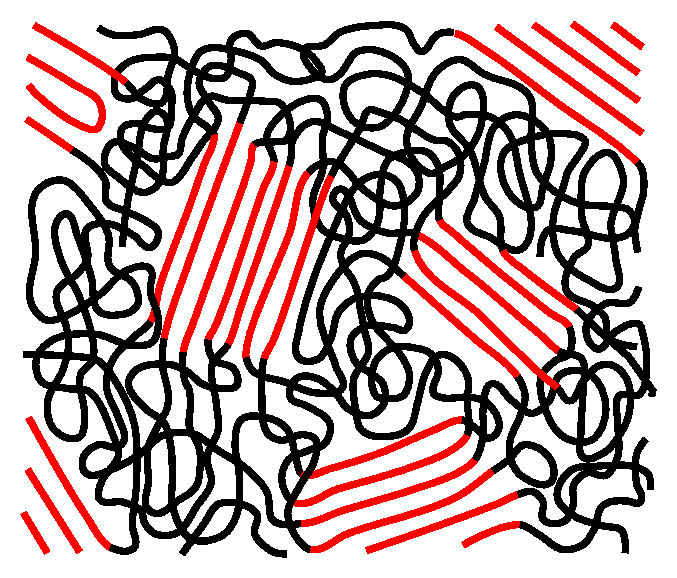
\includegraphics[width=.3\textwidth]{./static/rojtos-micella.pdf}
    \caption{Rojtos micella modell}
    \label{fig:micella}
  \end{figure}
  \tcbline

  A \textbf{kapcsolótábla modell} szerint egy nagy szilárd fázis alakul ki,
  amelyben lévő láncok a rész feletti és alatti amorf részen keresztül vannak
  összekapcsolva.
\end{question}


\begin{question}{
    Mutassa be a szferolitok szerkezetét és képződését. Hogyan befolyásolja a
    szferolitok mérete az anyag viselkedését? Hogyan tudjuk ezt megváltoztatni?
  }
  A szferolit mikroszkóp alatt látható \textbf{szuperkristály}. Gömbszerű
  szerkezet, nem csak polimerekben figyelhető meg. Az anyagban az
  \textbf{inhomogenitás} (csíra, góc, pl. szennyeződés) környékén indul meg a
  lamellák (\textbf{krisztallitok}) kialakulása. Kisszögű elágazások mentén
  lévő lamellacsoportulásokat \textbf{fibrilláknak} szokták hívni. Lehet sünis
  és kévés szerkezetű. Méretük a hőmérséklet változtatásával befolyásolható.
  Gyorsabb hűtéssel kisebb szferolitok alakulnak ki. Finomabb szerkezet esetén
  az anyagnak jobb mechanikai tulajdonságai lesznek. Szferolitképződés a
  csokinál is megfigyelhető.
  Méretük: $d = 5\,\mu\text{m} \dots \,\mathrm{mm}$.
\end{question}


\begin{question}{
    Hogyan befolyásolja a kristályos részarány a polimerek tulajdonságait? A
    szferolitos szerkezet mellett milyen szuperkristályos szerkezeteket ismer?
    Mutassa be ezeket röviden.
  }
  % Szuperkristályos szerkezetek:
  \begin{itemize}
    \item Transzkristályos szerkezet
          \begin{itemize}
            \item Gócok inhomogén elhelyezkedése miatt térben gátolt a
                  növekedés. (Ha sok góc egymás mellett van, akkor csak
                  hosszirányban tudnak nőni, tűs szerkezet alakul ki.)
                  Erősen anizotóp, rideg, de mechanikailag összességében
                  előnyös.
          \end{itemize}
    \item Fibrilláris szerkezet
          \begin{itemize}
            \item Szálhossz irányában nagy nyújtás hatásására nagy molekuláris
                  orientáció (irányulás) alakul ki. Húzásnak jól ellenáll,
                  nyírásnak nem. Modulus és szilárdságnövekedés, műszálak
                  tulajdonságai ezért jók.
          \end{itemize}
    \item Sish-kebab szerkezet
          \begin{itemize}
            \item Nagy belső orientációjú szerkezet, strapabíró, nagy
                  szilárdságú részek nem tudnak elcsúszni.
          \end{itemize}
    \item Összetett szerkezetek – Valóságban a szerkezetek keveredve jelennek
          meg.
  \end{itemize}
\end{question}


\begin{question}{
    Mutassa be a részben kristályos polimerek jellemző szerkezeti szintjeit.
  }
  \begin{itemize}
    \item Molekuláris szerkezet
    \item Nanoszerkezet (krisztallitok és amorf fázisok)
    \item Mezoszkópikus szerkezet (szuperkristályok, átmenen $nm$ és
          $\text{\textmu}m$ között)
    \item Finomszerkezet
    \item Makroszkópikus szerkezet
  \end{itemize}
\end{question}


\begin{question}{
    Mit nevezünk halmazállapotnak, fizikai állapotnak, illetve fázisnak? Gráf
    segítségével mutassa be a polimerek fizikai állapotai közötti lehetséges
    átmeneteket és a kapcsolódó jellemző hőmérsékleteket. Értelmezze a gráfot.
  }
  A polimereknél csak \textbf{szilárd} és \textbf{folyékony halmazállapot}
  jelentkezik, gáz nincsen. Nem szublimálnak, ezért nincsen szaguk. Nem
  desztillálhatóak, sem párologtathatóak. A \textbf{degradáció} az egész
  életüket végigkíséri.
  \tcbline

  \underline{\textbf{\textit{Fizikai állapotok:}}}
  \begin{multicols}{2}
    \begin{itemize}
      \item kristályos
      \item viszkózusan folyós
      \item nagyrugalmas amorf
      \item üvegesen amorf
    \end{itemize}
  \end{multicols}
  \tcbline

  \underline{\textbf{\textit{Fázis:}}} \\
  Az anyag olyan \textbf{lényegi része}, amelynek kémiai összetétele és fizikai
  állapota meegyezik (\textbf{egységes}). A fázisdomén egy termodinamikailag
  összefüggő területe az anyagnak.
  \tcbline

  \underline{\textbf{\textit{Fizikai állapotok közötti átmenetek:}}}
  \begin{figure}[H]
    \begin{tikzpicture}
      \draw[-to, ultra thick] (-7, -6) -- ++(0,12)
      node [above, black] {$T$, $H$ (entalpia)};

      \node[
        circle, draw, align=center, ultra thick
      ] (r1) at (0, 4) {Viszkózusan\\folyós};

      \node[
        circle, draw, align=center, ultra thick
      ] (r2) at (-3.5, -4) {Kristályos};

      \node[
        circle, draw, align=center, ultra thick
      ] (r3) at (2, 0) {Nagyrugalmas\\amorf};

      \node[
        circle, draw, align=center, ultra thick
      ] (r4) at (4, -4) {Üvegesen\\amorf};

      \draw [
      to-,
      ultra thick,
      cyan,
      postaction={
      decorate,
      decoration={
      raise=+1ex,
      text along path,
      text align=center,
      text=Krist{á}lyosod{á}s {$T_{kr}$}
      }
      }
      ] (r2) to [bend left=55] (r1);
      \draw [
      -to,
      ultra thick,
      cyan,
      postaction={
      decorate,
      decoration={
      raise=+1ex,
      text along path,
      text align=center,
      text=Krist{á}lyolvad{á}s {$T_{m}$}
      }
      }
      ] (r2) to [bend left] (r1);
      \draw [
      to-,
      ultra thick,
      cyan,
      postaction={
      decorate,
      decoration={
      raise=+1ex,
      text along path,
      text align=center,
      text=Hidegkrist{á}lyosod{á}s {$T_{hk}$}
      }
      }
      ] (r2) to [bend left] (r3);
      \draw [
      to-,
      ultra thick,
      cyan,
      postaction={
      decorate,
      decoration={
      raise=+1ex,
      text along path,
      text align=center,
      text={Ü}vegesed{é}s
      }
      }
      ] (r3) to [bend left] (r4);
      \draw [
        -to,
        ultra thick,
        cyan,
        postaction={
            decorate,
            decoration={
                raise=+1ex,
                text along path,
                text align=center,
                text={}{$T_g$}
              }
          }
      ] (r3) to [bend right] (r4);
      \draw [
      to-,
      ultra thick,
      cyan,
      postaction={
      decorate,
      decoration={
      raise=+1ex,
      text along path,
      text align=center,
      text=Foly{á}s
      }
      }
      ] (r1) to [bend left] (r3);
      \draw [
        -to,
        ultra thick,
        cyan,
        postaction={
            decorate,
            decoration={
                raise=+1ex,
                text along path,
                text align=center,
                text={}{$T_f$}
              }
          }
      ] (r1) to [bend right] (r3);

    \end{tikzpicture}
    \caption{Polimerek fizikai állapotai}
    \label{fig:poliphysics}
  \end{figure}
\end{question}


\begin{question}{
    Diagram segítségével mutassa be a lineáris a) amorf, b) részben kristályos
    polimerek fajtérfogat-változását a hőmérséklet függvényében. Hasonlítsa
    össze kismolekulájú anyagok viselkedésével. Adjon magyarázatot a változások
    okára.
  }
  Kismolekulák esetében a kitűntetett hőmérsékleti értékek konkrét értékek,
  polimereknél \textbf{intervallumok}. Kismolekulájú anygoknál az átmenet éles,
  polimereknél \textbf{lekerekítés} van. Kismolekuláknál megkülönböztetünk
  továbbá első- és másodrendű átalakulást.
  \tcbline

  \underline{\textbf{\textit{Nevezetes hőmérsékletek:}}}
  \begin{table}[H]
    \centering\begin{tabular}{r c l}
      $T_g$    & – & Üvegesedési átmeneti hőmérséklet \\
      $T_f$    & – & Folyási átmeneti hőmérséklet     \\
      $T_{kr}$ & – & Kristályosodási hőmérséklet      \\
      $T_m$    & – & Kristályolvadási hőmérséklet     \\
      $T_{hk}$ & – & Hidegkristáyosodási hőmérséklet  \\
    \end{tabular}
  \end{table}
  \tcbline

  \begin{figure}[H]
    \centering
    \begin{tikzpicture}
      \draw[ultra thick, -to] (-.5, 0) -- ++(8, 0)
      node [below right] {$T\; [\mathrm{K}]$};
      \draw[ultra thick, -to] (0,-.5) -- ++(0, 6)
      node [below left] {$v\; [\mathrm{cm^3/g}]$};

      \draw[domain=0:3, smooth, variable=\x, red, ultra thick]
      plot ({\x}, {1+.3*\x});
      \draw[domain=4:7, smooth, variable=\x, red, ultra thick]
      plot ({\x}, {.9*\x-1});

      \draw[red, ultra thick]
      (3,1.9) .. controls (3.33,2) and (3.33,2) .. (4,2.6);

      \draw[ultra thick, cyan, dashed]
      (3.5,0) node[below, black] {$T_g$} -- ++(0, 5);
      \draw[gray, thick, dashed] (3,0) -- ++(0, 5);
      \draw[gray, thick, dashed] (4,0) -- ++(0, 5);

      \draw[ultra thick, dashed, cyan]
      (5.5,0) node[below, black] {$T_f$} -- ++(0, 5);
      \draw[gray, thick, dashed] (5,0) -- ++(0, 5);
      \draw[gray, thick, dashed] (6,0) -- ++(0, 5);

      \draw[-to, ultra thick, yellow!50!black] (3.5,.25) -- ++(-2.5,0)
      node[midway, above, black] {Üvegesen};
      \draw[to-to, ultra thick, yellow!50!black] (3.5,.25) -- ++(2,0)
      node[midway, above, black] {Nagyrug.};
      \draw[-to, ultra thick, yellow!50!black] (5.5,.25) -- ++(1.5,0)
      node[midway, above, black] {Viszk.};

      \node[align=center] at (1.75,4) {\xcancel{\textmu B}\\ \xcancel{MB}};
      \node[align=center] at (4.5,4) {\textmu B\\ \xcancel{MB}};
      \node[align=center] at (6.5,4) {{\textmu B}\\ {MB}};
    \end{tikzpicture}
    \caption{Amorf anyagok fajtérfogatváltozása}
    \label{fig:vol-am}
  \end{figure}
  \tcbline

  \begin{figure}[H]
    \centering
    \begin{tikzpicture}[decoration={markings,
            mark= at position 0.5 with {\arrow{to}}}
      ]
      \draw[ultra thick, -to] (-.5, 0) -- ++(11, 0)
      node [below right] {$T\; [\mathrm{K}]$};
      \draw[ultra thick, -to] (0,-.5) -- ++(0, 7)
      node [below left] {$v\; [\mathrm{cm^3/g}]$};

      \draw[domain=0:3, smooth, variable=\x, red, ultra thick]
      plot ({\x}, {.5+.25*\x});
      \draw[domain=4:6, smooth, variable=\x, red, ultra thick]
      plot ({\x}, {-1.25+.75*\x});
      \draw[domain=8:9.5, smooth, variable=\x, red, ultra thick]
      plot ({\x}, {-1.25+.75*\x});

      \draw[red, ultra thick]
      (3,1.25) .. controls (3.5,1.375) and (3.5,1.375) .. (4,1.75);
      \draw[red, ultra thick, postaction={decorate}]
      (6,3.25) .. controls (7,3.5) and (7,3.5) .. (8,4.75);
      \draw[red, ultra thick, postaction={decorate}]
      (8,4.75).. controls (7,4.5) and (7,4.5) .. (6,3.25);

      \draw[ultra thick, cyan, dashed]
      (3.5,0) node[below, black] {$T_g$} -- ++(0, 6);
      \draw[gray, thick, dashed] (3,0) -- ++(0, 6);
      \draw[gray, thick, dashed] (4,0) -- ++(0, 6);

      \draw[ultra thick, dashed, cyan]
      (6.5,0) node[below, black] {$T_{kr}$} -- ++(0, 6);
      \draw[gray, thick, dashed] (6,0) -- ++(0, 6);
      \draw[gray, thick, dashed] (7,0) -- ++(0, 6);

      \draw[ultra thick, dashed, cyan]
      (8,0) node[below, black] {$T_m$} -- ++(0, 6);
      \draw[gray, thick, dashed] (7.5,0) -- ++(0, 6);
      \draw[gray, thick, dashed] (8.5,0) -- ++(0, 6);

      \draw[-to, ultra thick, yellow!50!black] (3.5,.25) -- ++(-2.5,0)
      node[midway, above, black] {Üvegesen};
      \draw[ultra thick, yellow!50!black] (3.5,.25) -- ++(4.5,0)
      node[midway, xshift=-7mm, above, black] {Nagyrug.};
      \draw[ultra thick, yellow!50!black] (8,.1) -- ++(0,.3);
      \draw[ultra thick, yellow!50!black] (3.5,.1) -- ++(0,.3);
      \draw[-to, ultra thick, yellow!50!black] (8,.25) -- ++(1.5,0)
      node[midway, above, black] {Viszk.};

      \draw[-to, ultra thick, yellow!50!black] (3.5,1.5) -- ++(-2.5,0)
      node[midway, above, black] {Kristályos};
      \draw[ultra thick, yellow!50!black] (3.5,1.5) -- ++(4.5,0);
      \draw[ultra thick, yellow!50!black] (8,1.35) -- ++(0,.3);
      \draw[-to, ultra thick, yellow!50!black] (8,1.5) -- ++(1.5,0)
      node[midway, above, black] {Viszk.};

      \draw[to-to, ultra thick, yellow!50!black] (8,5.5) -- ++(-1.5,0)
      node[midway, above, black]
      {\scriptsize$20${}$-${}$50^\circ\mathrm{C}$};

      \node[align=center] at (1.75,5) {\xcancel{\textmu B}\\ \xcancel{MB}};
      \node[align=center] at (5,5) {\textmu B\\ \xcancel{MB}};
      \node[align=center] at (9.5,5) {{\textmu B}\\ {MB}};
    \end{tikzpicture}
    \caption{Részben kristályos anyagok fajtérfogatváltozása}
    \label{fig:vol-cr}
  \end{figure}
\end{question}


\begin{question}{
    Ismertesse a polimerek fizikai állapotait (főbb jellegzetességek). Hol,
    hogyan és miért jelennek meg átmenetek a fizikai állapotok között?
  }
  Minden esetben próbáljuk \textbf{elkerülni} az \textbf{üvegesedési
    hőmérséklet-tartományt}:
  \begin{table}[H]
    \centering\begin{tabular}{| l | r |}
      \hline
      Lineáris amorf     & $T_g$ alatt (üveges)        \\
      Részben kristályos & $T_m$ alatt                 \\
      Sűrűn térhálós     & $T_g$ alatt (üveges)        \\
      Ritkán térhálós    & $T_g$ felett (nagyrugalmas) \\
      \hline
    \end{tabular}
    \caption{Polimerek felhasznánási tartománya}
    \label{table:use}
  \end{table}
\end{question}


%%%%%%%%%%%%%%%%%%%%%%%%%%%%%%%%%%%%%%%%%%%%%%%%%%%%%%%%%%%%%%%%%%%%%%%%%%%%%%%
\newcommand\angstrom{\mbox{\normalfont\AA}}
\newcommand\namebond[4][5pt]{\chemmove{\path(#2)--(#3)node[midway,sloped,yshift=#1]{#4};}}

\newcommand\arcbetweennodes[3]{%
  \pgfmathanglebetweenpoints{
    \pgfpointanchor{#1}{center}
  }{
    \pgfpointanchor{#2}{center}
  }%
  \let#3\pgfmathresult
}

\newcommand\arclabel[6][to-to,shorten <=1pt,shorten
  >=1pt]{%
  \chemmove{%
    \arcbetweennodes{#4}{#3}\anglestart
    \arcbetweennodes{#4}{#5}\angleend
    \draw[#1]([shift=(\anglestart:#2)]#4)arc(\anglestart:\angleend:#2);
    \pgfmathparse{(\anglestart+\angleend)/2}\let\anglestart\pgfmathresult
    \node[
      shift=(\anglestart:#2+1pt)#4,
      anchor=\anglestart+180,
      rotate=\anglestart+90,
      inner sep=0pt,
      outer sep=0pt
    ]at(#4){#6};}}

\begin{question}{
    Mit nevezünk konformációnak? Mutassa be a molekulaláncok lehetséges
    hőmozgásait. Mit nevezünk kígyózó mozgásnak?
  }
  A \textbf{konformációs izomerek} elforgatással keletkeznek spontán, vagy
  mechanikai ráhatás következtében.
  \begin{center}
    \chemfig[
    angle increment=35.25,
    atom sep=2em,
    bond style={line width=1pt,red}
    ]{-[1]-[-1]@{1}-[1]@{2}-[-1]@{3}-[1]-[-1]-[1]-[-1]-[1]-[-1]-[1]}
    \arclabel{0.5cm}{1}{2}{3}{\footnotesize109.5\textdegree}
  \end{center}
  \[
    \downarrow
  \]
  \begin{center}
    \chemfig[
    angle increment=35.25,
    atom sep=2em,
    bond style={line width=1pt,red}
    ]{-[1]-[-1]-[1]-[::-40]-[1]-[-1]-[::+50]-[-1]-[1]-[-1]-[1]}
  \end{center}
  \tcbline

  \underline{\textbf{\textit{Hőmozgások:}}} \\
  A rendszer entalpiájától függ az intenzitása. Fajtái:
  \begin{itemize}
    \item \textbf{Atomcsoportok mozgása} – kötésszögek atomi szinten
          megváltoznak
    \item \textbf{Szegmensmozgások} (\textmu B – Mikro-Brown mozgások)
          \begin{itemize}
            \item molekulák egyes részei konformációs változást okozva
                  elmozdulnak
            \item a \textbf{szegmens} a molekula termodinamikailag összefüggő
                  egysége
          \end{itemize}
    \item \textbf{Makro-Brown mozgások} (MB)
          \begin{itemize}
            \item molekulák középpontja is elcsúszik
          \end{itemize}
  \end{itemize}

  \tcbline
  \underline{\textbf{\textit{Kígyózó mozgás:}}} \\
  \textbf{Áthurkolódások} olyan virtuális csövet hoznak létre, amiben a
  molekula el tud fordulni, mozdulni. \textbf{Reptációnak} is szokás nevezni.
\end{question}


\begin{question}{
    Mutassa be a molekulaláncok mechanikai behatásra történő mozgásait. Mutassa
    be részletesen a polimerek deformációkomponenseit! Milyen viselkedési
    jelenségeket mutatnak ezek az anyagok?
  }
  Viszkoelasztikus anyagoknál \textbf{rugalmas} (elasztikus) és
  \textbf{viszkózus} viselkedés is megfigyelhető. Összetett viselkedésüket
  ideális tulajdonságok kombinációjaként írjuk le. Az összdeformáció 3
  komponensből tevődik össze:
  \begin{itemize}
    \item $\varepsilon_{pr}$ – \textbf{pillanatnyi rugalmas} komponens
          \begin{itemize}
            \item Hooke-törvényt ($\sigma = E \cdot \varepsilon$) követő
                  ideális rugó.
            \item Atomtávolságok és vegyértékszögek megváltozása.
            \item Mechanikailag és termodinamikailag is reverzibilis.
          \end{itemize}
    \item $\varepsilon_{m}$ – \textbf{maradó} deformáció
          \begin{itemize}
            \item Newton-törvényt ($\sigma = \eta \cdot \dot{\varepsilon}$)
                  követő ideális viszkózus elem.
            \item Molekulaláncok egymáshoz képest elcsúsznak.
            \item Mechanikailag és termodinamikailag is irreverzibilis.
          \end{itemize}
    \item $\varepsilon_{kr}$ – \textbf{késleltetett rugalmas} komponens
          \begin{itemize}
            \item Kelvin-Voigt elem (rugó és viszkózus elem párhuzamos
                  kapcsolása).
            \item Molekulaláncok ki- él visszagöngyölődése. \\
                  (szegmensmozgások, konformációváltozások)
            \item Mechanikailag reverzibilis, de termodinamikailag nem.
            \item Hiszterézishurok jellemzi.
          \end{itemize}
  \end{itemize}
  A viselkedés a \textbf{Burgers-féle négyparaméteres modellel} írható le.
\end{question}


\begin{question}{
    Mutassa be, hogyan modellezhetők az egyes deformációkomponensek
    viszkoelasztikus anyagoknál! (Modellek, vonatkozó törvények, paraméterek).
  }
  A viselkedés a \textbf{Burgers-féle négyparaméteres modellel} írható le.
  \begin{figure}[H]
    % By Davius - Own work, Public Domain, https://commons.wikimedia.org/w/index.php?curid=11329412
    \centering
    \begin{tikzpicture}[thick]
      \fill [pattern = north west lines] (0,-1) rectangle ++(-.2,2);
      \draw[thick] (0,-1) -- ++(0,2);

      \draw (0, 0)
      to[spring=$E_1$] ++(1.5, 0)
      to[damper=$\eta_1$] ++(2, 0)
      to[short] ++(0,1)
      to[spring=$E_2$] ++(2,0)
      to[short] ++(0,-1)
      to[short] ++(.5,0);
      \draw (3.5,0)
      to[short] ++(0,-1)
      to[damper=$\eta_2$] ++(2,0)
      to[short] ++(0,1);
    \end{tikzpicture}
    % 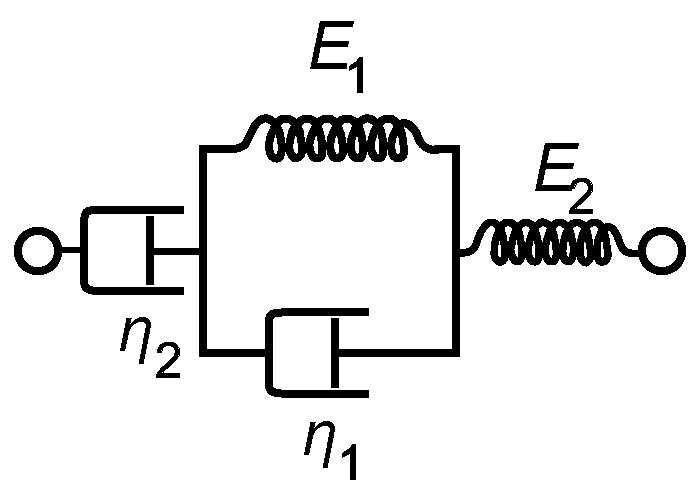
\includegraphics[width=.4\textwidth]{./static/Burgers_model.pdf}
    \caption{Burgers-modell}
    \label{fig:Burgers}
  \end{figure}
\end{question}


\begin{question}{
    Mit jelent az, hogy egy anyag viszkoelasztikus, illetve lineárisan
    viszkoelasztikus? Hogyan csoportosíthatók a különböző mechanikai
    vizsgálatok polimereknél a gerjesztés típusa szerint? Melyiknél mi a
    gerjesztés és milyen választ várunk rá?
  }
  Viszkoelasztikus anyagoknál \textbf{rugalmas} (elasztikus) és
  \textbf{viszkózus} viselkedés is megfigyelhető. Összetett viselkedésüket
  ideális tulajdonságok kombinációjaként írjuk le.
  \tcbline

  \textbf{Lineárisan viszkoelasztikus} anyagoknál a szakítógörbéjüknek van
  egyenes szakasza, vagyis itt érvényes a Hooke-törvény. Általában ebben a
  tartományban vizsgálódunk, hiszen itt könnyű számolni.
  \tcbline

  \underline{\textbf{\textit{Mechanikai vizsgálatok:}}}
  \begin{itemize}
    \item Állandó terhelés:
          \begin{itemize}
            \item kúszásvizsgálat – állandó feszültség
            \item feszültségrelaxáció – állandó alakváltozás
          \end{itemize}
    \item Allándó sebesség:
          \begin{itemize}
            \item szakítóvizsgálat
          \end{itemize}
    \item ciklikus terhelés
          \begin{itemize}
            \item DMA vizsgálat
            \item fárasztóvizsgálat
          \end{itemize}
    \item Pillanatszerű:
          \begin{itemize}
            \item ütővizsgálat
          \end{itemize}
  \end{itemize}
\end{question}


\begin{question}{
    Mutassa be a polimerek szakítóvizsgálatának menetét és a kapott eredmények
    kiértékelési módszerét. Mit nevezünk mérnöki feszültségnek? Mi a fajlagos
    nyúlás? Milyen jellegzetes pontjai vannak a görbének?
  }
  \textbf{Szakítóvizsgálat} során a polimer próbatest \textbf{állandó
    sebességű} húzó igénybevételnek van kitéve, a feszültség értéke
  folyamatosan változik, melyet az alakváltozás függvényében vizsgálunk. A
  próbatest \textbf{piskóta} alakú, szabványos méretű.
  \tcbline

  A \textbf{mérnöki feszültség} az erő és a kezdeti keresztmetszet hányadosa:
  \[
    \sigma = \frac{F}{A_0}
  \]
  A \textbf{fajlagos nyúlás} a megnyúlás és a kezdeti hossz hányadosa:
  \[
    \varepsilon = \frac{\Delta l}{l_0}
  \]

  \tcbline
  \underline{\textbf{\textit{A görbe nevezetes pontjai:}}}
  \begin{itemize}
    \item nevezetes feszültségek:
          \begin{itemize}
            \item $\sigma_M$ – húzószilárdság (első lokális maximum)
            \item $\sigma_B$ – szakítószilárdság (szakadás pillanatában mért)
            \item $\sigma_Y$ – folyási feszültség
                  (utána a nyúlás a feszültség növekedése nélkül növekszik)
          \end{itemize}
    \item nevezetes nyúlások:
          \begin{itemize}
            \item $\varepsilon_M$ – nyúlás maximális erőnél
            \item $\varepsilon_B$ – szakadási nyúlás
          \end{itemize}
  \end{itemize}
\end{question}


\begin{question}{
    Mit jelent a polimerek húzási rugalmassági modulusa, milyen módszerekkel
    lehet ezt meghatározni egy szakítógörbéből? Miért van szükség eltérő
    módszerekre ehhez?
  }
  A húzási rugalmassági modulus a \textbf{szakítógörbe meredeksége}. A
  feszültség és az alakváltozás közötti kapcsolatot fejezi ki. Megmutatja, hogy
  adott terhelésre milyen nyúlással reagál az anyag. Fajtái:
  \begin{multicols}{3}
    \begin{itemize}
      \item kezdeti rug. mod.
      \item húr mod.
      \item érintő mod.
    \end{itemize}
  \end{multicols}
  Azért van szükség rájuk, mert a rugalmassági modulus \textbf{nem állandó} a
  szakítógörbe mentén (, meredeksége változik).
\end{question}


\begin{question}{
    Milyen eltérések vannak a polimerek és a fémek mechanikai viselkedése
    között? Jellegzetes szakítógörbék segítségével mutassa be az eltéréseket,
    valamint a szakítógörbék nevezetes pontjait és szakaszait.
  }
  Fémes szerkezeti anyagoknál a folyási feszültség egy éles határ
  (folyáshatár): alatta rugalmas, míg felette képlékeny alakváltozás
  jelentkezik. A viszkoelasztikus viselkedésű polimereknél már rendszerint
  \textbf{kis feszültségeknél} is \textbf{maradó alakváltozások} alakulnak ki,
  tehát folyáshatár nincsen, sőt a gyakorlatban bizonyos polimereknél fel sem
  lép a folyási jelenség.
\end{question}


\begin{question}{
    Mi a dinamikus termomechanikai analízis lényege? Mi a gerjesztés? Mi erre a
    válasz? (egyenletek!) Hogyan végzünk el egy ilyen mérést? Komplex számsíkon
    mutassa be és értelmezze, hogy mit jelent a tárolási és a veszteségi
    modulus, valamint a veszteségi tényező.
  }
  A DMA (dinamikus mechanikai analízis) egy \textbf{fárasztóvizsgálat}. Egy $4
    \cross 10 \cross 60 \, \mathrm{mm}$ méretű hasábot \textbf{ciklikusan}
  (szinuszosan) \textbf{terheljük} és a feszültséget, alakváltozást az idő
  függvényében vizsgáljuk. A próbatestet csavaró vagy nyíró igénybevétellel is
  terhelhetjük. Az alakváltozás és a feszültség között fáziskésés figyelhető
  meg:
  \begin{align*}
    \varepsilon(t) & = \varepsilon_0 \cdot \sin(\omega t)
    \\
    \sigma(t)      & = \sigma_0 \cdot \sin(\omega t + \delta)
    \\
                   & = \sigma_0 \left(
    \cos \delta \sin(\omega t) +
    \sin \delta \cos(\omega t)
    \right)
    \\
                   & = \sigma'_0 \sin(\omega t) + \sigma''_0 \cos(\omega t)
  \end{align*}
  Kis rezgés esetén alkalmazható a Hooke-törvény:
  \[
    E^*(t)
    = \frac{\sigma(t)}{\varepsilon_0}
    = \frac{\sigma'_0}{\varepsilon_0} \cdot \sin \left( \omega t \right)
    + \frac{\sigma''_0}{\varepsilon_0} \cdot \cos \left( \omega t \right)
    = E' \cdot \sin \left( \omega t \right)
    + E'' \cdot \cos \left( \omega t \right)
  \]
  \begin{itemize}
    \item $E^*(t)$ – Komplex rugalmassági modulus
    \item $E'$ – Tárolási modulus (ideálisan rugalmas)
    \item $E''$ – Veszteségi modulus (ideálisan viszkózus)
  \end{itemize}
  \begin{figure}[H]
    \centering
    \begin{tikzpicture}
      \coordinate (origo) at (0, 0);
      \coordinate (re) at (4, 0);
      \coordinate (im) at (0, 3);
      \coordinate (sum) at (4, 3);

      \draw[-to, ultra thick, black] (-0.5, 0) -- (4.5, 0);
      \node[below right] at (4.5, 0) {Re};
      \draw[-to, ultra thick, black] (0, -0.5) -- (0, 3.5);
      \node[above left] at (0, 3.5) {Im};

      \draw[-latex, cyan, ultra thick] (origo) -- (re)
      node[below, midway, black] {$E'$};

      \draw[-latex, magenta, ultra thick] (re) -- (sum)
      node[right, midway, black] {$E''$};

      \draw[-latex, red, ultra thick] (origo) -- (sum)
      node[above left, midway, black] {$E^*$};

      \draw pic[
          -to,
          ultra thick,
          "$\delta$",
          draw=yellow!50!black,
          angle radius=40,
          angle eccentricity=.6
        ]
        {angle = re--origo--sum};
    \end{tikzpicture}
    \caption{Komplex rugalmassági modulus ábrázolása}
    \label{fig:complexE}
  \end{figure}
  Ha $\delta < 45^\circ$, akkor inkább szilárd, ha $\delta>45^\circ$, akkor
  inkább folyékony. Veszteségi tényező:
  \[
    d:= \tan \delta = \frac{E''}{E'}
  \]
\end{question}


\begin{question}{
    Mutassa be és hasonlítsa össze az amorf lineáris polimerek és a gyengén
    térhálós elasztomerek DMA görbéit. Jelölje be az egyes fázisok fizikai
    állapotait, és a jellemző átmeneti hőmérsékleteket. Milyen
    hőmérséklettartományban használjuk ezeket az anyagokat?
  }
  Mindenképpen elkerüljük az üvegesedési tartományt. A hőre lágyuló amorf
  anyagokat $T_g$ alatt, az elasztomereket $T_g$ felett alkalmazzuk.
  \begin{figure}[H]
    \centering
    \hfill
    \begin{subfigure}[b]{0.49\textwidth}
      \centering
      \begin{tikzpicture}[ultra thick]
        % Coordinate system
        \draw[to-to] (0,5) node [above] {
          \color{yellow!50!black}{$E'$}
          \color{cyan!50!black}{$E''$}
        }
        -- (0,0)
        -- (7,0); %node [below right] {$T$};

        \draw[gray, thick, dashed] (3, 4.5)
        -- ++(0,-4.5) node[below, black] {$T_g$};
        \draw[gray, thick, dashed] (5, 4.5)
        -- ++(0,-4.5) node[below, black] {$T_f$};
        \draw[gray, thick, dashed] (6.5, 4.5)
        -- ++(0,-4.5) node[below, black] {$T_d$};

        \draw[yellow!50!black] (0,4)
        -- ++(.5,0)
        -- ++(.25, 0) -- ++(0,-.1)
        -- ++(.25, 0) -- ++(0,-.1)
        -- ++(.25, 0) -- ++(0,-.1)
        -- ++(.25, 0) -- ++(0,-.1)
        -- ++(.5,0)
        .. controls (3,3.6) and (3,1.2) .. (4,1)
        .. controls (5,.8) and (6.3,.6) .. (6.4,0);

        \draw[cyan!50!black] (0,.35)
        -- ++(2,0)
        .. controls (2.5,.35) and (2.5,1.25) .. (3,1.25)
        .. controls (3.5,1.25) and (3.5,.52) .. (5,.5)
        .. controls (5.75,.53) and (6,1) .. (6.45,4);

        \draw[|-to, gray] (2.5, 2) -- (.5,2)
        node[midway, black, align=center]
        {\scriptsize Felhasználási\\ \scriptsize tartomány};
        \draw[|-to, gray] (3.5, 2) -- (4.75,2)
        node[midway, black, align=center]
        {\scriptsize Feldolg.\\ \scriptsize tart.};

        \node[align=center] at (1.5,4.5)
        {\scriptsize\xcancel{\textmu B}\\ \scriptsize\xcancel{MB}};
        \node[align=center] at (4,4.5)
        {\scriptsize\textmu B\\ \scriptsize\xcancel{MB}};
        \node[align=center] at (5.75,4.5)
        {\scriptsize\textmu B\\ \scriptsize{MB}};
      \end{tikzpicture}
      \caption{Amorf termoplasztikus anyagok}
    \end{subfigure}
    \hfill
    \begin{subfigure}[b]{0.49\textwidth}
      \centering
      \begin{tikzpicture}[ultra thick]
        % Coordinate system
        \draw[to-to] (0,5) node [above] {
          \color{yellow!50!black}{$E'$}
          \color{cyan!50!black}{$E''$}
        }
        -- (0,0)
        -- (7,0); %node [below right] {$T$};

        \draw[gray, thick, dashed] (2.5, 4.5)
        -- ++(0,-4.5) node[below, black] {$T_g$};
        \draw[gray, thick, dashed] (6.5, 4.5)
        -- ++(0,-4.5) node[below, black] {$T_d$};

        \draw[yellow!50!black] (0,4)
        .. controls (4,4) and (1,.7) .. (5,.5)
        -- ++(1.5, -0.075);

        \draw[cyan!50!black] (0,.35)
        -- ++(1.5,0)
        .. controls (2,.35) and (2,1) .. (2.5,1)
        .. controls (3,1) and (3,.333) .. (4,.3)
        -- ++(2.5,-.1);

        \draw[|-to, gray] (3, 3) -- (5,3)
        node[midway, black, align=center]
        {\scriptsize Felhasználási \\ \scriptsize tartomány};

        \node[align=center] at (1.25,4.5)
        {\scriptsize\xcancel{\textmu B}\\ \scriptsize\xcancel{MB}};
        \node[align=center] at (4.5,4.5)
        {\scriptsize\textmu B\\ \scriptsize\xcancel{MB}};
      \end{tikzpicture}
      \caption{Ritkán térhálós elasztomerek}
    \end{subfigure}
    \hfill
    \caption{Lineáris amorf és elasztomerek összehasonlítása}
    \label{fig:comp1}
  \end{figure}
\end{question}


\begin{question}{
    Mutassa be és hasonlítsa össze a részben kristályos lineáris polimerek és a
    sűrűn térhálós duromerek DMA görbéit. Jelölje be az egyes fázisok fizikai
    állapotait, és a jellemző átmeneti hőmérsékleteket. Milyen
    hőmérséklettartományban használjuk ezeket az anyagokat?
  }
  Egyes részben kristályos anyagokat $T_g$ alatt, másokat $T_g$ felett
  használjuk fel. Duromerek felhasználási tartománya $T_g$ alatt van, ezért
  előnyös, ha az magas. ($\chi\%$ – kristályos részarány, $\rho\%$ – térháló
  sűrűség)
  \begin{figure}[H]
    \centering
    \hfill
    \begin{subfigure}[b]{0.49\textwidth}
      \centering
      \begin{tikzpicture}[ultra thick]
        % Coordinate system
        \draw[to-to] (0,5) node [above] {
          \color{yellow!50!black}{$E'$}
          \color{cyan!50!black}{$E''$}
        }
        -- (0,0)
        -- (7,0); %node [below right] {$T$};

        \draw[gray, thick, dashed] (2, 4.5)
        -- ++(0,-4.5) node[below, black] {$T_g$};
        \draw[gray, thick, dashed] (3.75, 4.5)
        -- ++(0,-4.5) node[below, black] {$T_f$};
        \draw[gray, thick, dashed] (5.5, 4.5)
        -- ++(0,-4.5) node[below, black] {$T_m$};
        \draw[gray, thick, dashed] (6.5, 4.5)
        -- ++(0,-4.5) node[below, black] {$T_d$};

        \draw[yellow!50!black!50] (1,4)
        .. controls (2,4) and (2,2.3) .. (3,2.25);
        \draw[yellow!50!black!50] (1,4)
        .. controls (2,4) and (2,2.55) .. (3,2.5);
        \draw[yellow!50!black!50] (1,4)
        .. controls (2,4) and (2,2.8) .. (3,2.75);
        \draw[yellow!50!black!50] (1,4)
        .. controls (2,4) and (2,3.3) .. (3,3.25);
        \draw[yellow!50!black!50] (1,4)
        .. controls (2,4) and (2,3.55) .. (3,3.5);

        \draw[yellow!50!black] (0,4)
        -- ++(1,0)
        .. controls (2,4) and (2,3.1) .. (3,3)
        -- ++(1.5,-.15)
        .. controls (5,2.8) and (6,2.5) .. (6.2,0);

        \draw[cyan!50!black] (0,.35)
        -- ++(1,0)
        .. controls (1.5,.35) and (1.5,1.25) .. (2,1.25)
        .. controls (2.5,1.25) and (2.5,.52) .. (4,.5)
        .. controls (5.75,.53) and (6,1) .. (6.45,4);

        \draw[|-to, gray] (5.25, 2) -- (4,2)
        node[midway, black, align=center]
        {\scriptsize Felh.\\ \scriptsize tart.};

        \draw[-to, gray] (3, 2) -- (3,3.75)
        node[below right, black]{\scriptsize $\chi\%$};

        \node[align=center] at (1,4.5)
        {\scriptsize\xcancel{\textmu B}\\ \scriptsize\xcancel{MB}};
        \node[align=center] at (2.875,4.5)
        {\scriptsize\textmu B\\ \scriptsize\xcancel{MB}};
        \node[align=center] at (4.625,4.5)
        {\scriptsize\textmu B\\ \scriptsize\xcancel{MB}};
        \node[align=center] at (6,4.5)
        {\scriptsize\textmu B\\ \scriptsize{MB}};
      \end{tikzpicture}
      \caption{Részben kristályos polimerek}
    \end{subfigure}
    \hfill
    \begin{subfigure}[b]{0.49\textwidth}
      \centering
      \begin{tikzpicture}[ultra thick]
        % Coordinate system
        \draw[to-to] (0,5) node [above] {
          \color{yellow!50!black}{$E'$}
          \color{cyan!50!black}{$E''$}
        }
        -- (0,0)
        -- (7,0); %node [below right] {$T$};

        \draw[gray, thick, dashed] (4.5, 4.5)
        -- ++(0,-4.5) node[below, black] {$T_g$};
        \draw[gray, thick, dashed] (6.5, 4.5)
        -- ++(0,-4.5) node[below, black] {$T_d$};

        \draw[yellow!50!black!50] (3,4)
        .. controls (5,4) and (4,2.6) .. (6.5,2.5);
        \draw[yellow!50!black!50] (3,4)
        .. controls (5,4) and (4,2.35) .. (6.5,2.25);
        \draw[yellow!50!black!50] (3,4)
        .. controls (5,4) and (4,1.95) .. (6.5,1.75);
        \draw[yellow!50!black!50] (3,4)
        .. controls (5,4) and (4,1.6) .. (6.5,1.5);

        \draw[-to, gray] (5.5, 1.25) -- (5.5,3.25)
        node[below right, black]{\scriptsize $\rho\%$};

        \draw[yellow!50!black] (0,4)
        -- ++(3,0)
        .. controls (5,4) and (4,2.2) .. (6.5,2);

        \draw[cyan!50!black] (0,.35)
        -- ++(3.5,0)
        .. controls (4,.35) and (4,1.25) .. (4.5,1.25)
        .. controls (5,1.25) and (5,.5) .. (5.5,.5)
        -- ++(1,0);

        \draw[|-to, gray] (4, 2) -- ++(-1.5,0)
        node[midway, black, align=center]
        {\scriptsize Felh. \\ \scriptsize tart.};

        \node[align=center] at (2,4.5)
        {\scriptsize\xcancel{\textmu B}\\ \scriptsize\xcancel{MB}};
        \node[align=center] at (5.5,4.5)
        {\scriptsize\textmu B\\ \scriptsize\xcancel{MB}};
      \end{tikzpicture}
      \caption{Sűrűn térhálós duromerek}
    \end{subfigure}
    \hfill
    \caption{Részben kristályos anyagok és duromerek összehasonlítása}
    \label{fig:comp2}
  \end{figure}
\end{question}


\begin{question}{
    Mi a kúszás (polimerek esetén)? Adjon műszaki példákat. Mutassa be a kúszás
    gerjesztés- és válaszfüggvényét, mutassa be a kúszást leíró modellt a)
    amorf lineáris és b) gyengén térhálós polimerek esetén.
  }
  A kúszás (nyúlásrelaxáció) vizsgálat egy statikus vizsgálat, ahol a
  próbatestre ugrásszerűen egy bizonyos időre \textbf{állandó nagyságú
    feszülséget} kapcsolunk. Megfigyelhetjük, hogy a próbatest
  \textbf{alakváltozása} az idő függvényében \textbf{folyamatosan nő}. Pl.:
  polc lehajlása.
  \tcbline

  \underline{\textbf{\textit{Modellek:}}}

  \vspace{1em}
  \textbf{\textit{Hooke-törvényt követő rugó:}}
  \[
    \sigma = E \cdot \varepsilon
    \quad \rightarrow \quad
    \varepsilon_0 = \frac{\sigma_0}{E}
  \]
  \begin{figure}[H]
    \centering
    \begin{tikzpicture}[scale=.75,decoration={markings,
            mark= at position 0.25 with {\arrow{to}},
            mark= at position 0.5 with {\arrow{to}},
            mark= at position 0.75 with {\arrow{to}},
          }
      ]

      \draw[to-to, ultra thick]
      (0,3) node[below right] {$\sigma$} --
      ++(0,-3) --
      ++(5.1,0) node[below left] {$t$};
      \draw[to-to, ultra thick]
      (0,-1) node[below right] {$\varepsilon$} --
      ++(0,-3) --
      ++(5.1,0) node[below left] {$t$};

      \draw[ultra thick, yellow!50!black, postaction={decorate}]
      (0,0) --
      ++(1, 0) [postaction={decorate}] --
      ++(0, 1.5) --
      ++(3, 0) --
      ++(0,-1.5) --
      ++(1, 0);
      \draw[ultra thick, yellow!50!black, postaction={decorate}]
      (0,-4) --
      ++(1, 0) [postaction={decorate}] --
      ++(0, 1.5) --
      ++(3, 0) --
      ++(0,-1.5) --
      ++(1, 0);

      \draw[to-to, ultra thick]
      (8,-1) node[below right] {$\sigma$} --
      ++(0,-3) --
      ++(3,0) node[below left] {$\varepsilon$};

      \draw[ultra thick, yellow!50!black]
      (8,-4) -- ++(2.25,2.25);

      \coordinate (A) at (9, -3);
      \coordinate (B) at (10, -2);
      \coordinate (C) at (10.5, -3);

      \draw[thick, gray, dashed] (A) -- (C);

      \draw pic[
          -to,
          ultra thick,
          "$\alpha$",
          draw=red,
          angle radius=30,
          angle eccentricity=.6
        ]
        {angle = C--A--B};

      \fill [pattern = north west lines] (8.5,2.8) rectangle ++(2,.2);
      \draw[thick] (8.5,2.8) -- ++(2,0);

      \draw (9.5,2.8)
      to[spring=$E$, thick] ++(0,-2);
    \end{tikzpicture}
    \caption{Rugó modell}
    \label{fig:spring}
  \end{figure}

  \textbf{\textit{Ideális viszkózus elem:}}
  \[
    \sigma = \eta \cdot \dot{\varepsilon}
    \quad \rightarrow \quad
    \varepsilon(t) = \frac{\sigma_0}{\eta} \cdot t
  \]
  \begin{figure}[H]
    \centering
    \begin{tikzpicture}[scale=.75,decoration={markings,
            mark= at position 0.25 with {\arrow{to}},
            mark= at position 0.5 with {\arrow{to}},
            mark= at position 0.75 with {\arrow{to}},
          }
      ]

      \draw[to-to, ultra thick]
      (0,3) node[below right] {$\sigma$} --
      ++(0,-3) --
      ++(5.1,0) node[below left] {$t$};
      \draw[to-to, ultra thick]
      (0,-1) node[below right] {$\varepsilon$} --
      ++(0,-3) --
      ++(5.1,0) node[below left] {$t$};

      \draw[ultra thick, yellow!50!black, postaction={decorate}]
      (0,0) --
      ++(1, 0) [postaction={decorate}] --
      ++(0, 1.5) --
      ++(3, 0) --
      ++(0,-1.5) --
      ++(1, 0);
      \draw[ultra thick, yellow!50!black, postaction={decorate}]
      (0,-4) --
      ++(1,0) --
      ++(3,1.5) --
      ++(1,0);

      \draw[to-to, ultra thick]
      (8,-1) node[below right] {$\sigma$} --
      ++(0,-3) --
      ++(3,0) node[below left] {$\dot{\varepsilon}$};

      \draw[ultra thick, yellow!50!black]
      (8,-4) -- ++(2.25,2.25);

      \coordinate (A) at (9, -3);
      \coordinate (B) at (10, -2);
      \coordinate (C) at (10.5, -3);

      \draw[thick, gray, dashed] (A) -- (C);

      \draw pic[
          -to,
          ultra thick,
          "$\alpha$",
          draw=red,
          angle radius=30,
          angle eccentricity=.6
        ]
        {angle = C--A--B};

      \fill [pattern = north west lines] (8.5,2.8) rectangle ++(2,.2);
      \draw[thick] (8.5,2.8) -- ++(2,0);

      \draw (9.5,2.8)
      to[damper=$\eta$, thick] ++(0,-2);
    \end{tikzpicture}
    \caption{Viszkózus elem modell}
    \label{fig:visc}
  \end{figure}

  \textbf{\textit{Kelvin-Voigt elem:}}
  \begin{gather*}
    \sigma = \sigma_1 + \sigma_2
    \hspace{2.5em}
    \varepsilon = \varepsilon_1 = \varepsilon_2
    \\
    \sigma = E \cdot \varepsilon + \eta \cdot \dot{\varepsilon}
    \\
    \varepsilon(t) = \frac{\sigma_0}{E} \left(
    1 - e^{\sfrac{-t}{\tau}} \right)
    \\
    \tau = \eta/E \; \rightarrow \text{ retardációs idő}
  \end{gather*}
  \begin{figure}[H]
    \centering
    \begin{tikzpicture}[ultra thick, scale=.75, decoration={markings,
            mark= at position 0.25 with {\arrow{to}},
            mark= at position 0.75 with {\arrow{to}},
          }
      ]

      \draw[to-to, ultra thick]
      (0,3) node[below right] {$\sigma$} --
      ++(0,-3) --
      ++(5.1,0) node[below left] {$t$};
      \draw[to-to, ultra thick]
      (0,-1) node[below right] {$\varepsilon$} --
      ++(0,-3) --
      ++(5.1,0) node[below left] {$t$};

      \draw[ultra thick, yellow!50!black, postaction={decorate}]
      (0,0) --
      ++(.5, 0) [postaction={decorate}] --
      ++(0, 1.5) --
      ++(2.2, 0) --
      ++(0,-1.5) --
      ++(1.8, 0);
      \draw[ultra thick, yellow!50!black, postaction={decorate}]
      (0,-4) --
      ++(.5,0) to[bend left]
      ++(2.2,1.5) to[bend right]
      ++(1.8,-1.3);

      \draw[to-to, ultra thick]
      (8,-1) node[below right] {$\sigma$} --
      ++(0,-3) --
      ++(3,0) node[below left] {${\varepsilon}$};

      \draw[ultra thick, yellow!50!black, postaction={decorate}]
      (8,-4)
      to[bend right] ++(2.25,1.75)
      to[bend right] (8,-4);

      \fill [pattern = north west lines] (8.5,2.8) rectangle ++(2,.2);
      \draw[thick] (8.5,2.8) -- ++(2,0);

      \begin{scope}[thick]
        \draw (9.5,2.8)
        to[short] ++(0,-.25)
        to[short] ++(-.75,0)
        to[damper=$\eta$, thick] ++(0,-2)
        to[short] ++(.75,0)
        to[short] ++(0,-.25);
        \draw (9.5,2.8)
        to[short] ++(0,-.25)
        to[short] ++(.75,0)
        to[spring=$E$, thick] ++(0,-2)
        to[short] ++(-.75,0)
        to[short] ++(0,-.25);
      \end{scope}
    \end{tikzpicture}
    \caption{Kelvin-Voigt elem}
    \label{fig:kv}
  \end{figure}
  \tcbline

  \underline{\textbf{\textit{Amorf lineáris anyagok kúszása:}}} \\
  Az amorf termoplasztikus polimereket a \textbf{Burgers-modell} segítségével
  írhatjuk le. Ez a modell az előbbi 3 elem összekapcsolásával valósul meg,
  négyparaméteres modell.
  \begin{gather*}
    \varepsilon
    = \varepsilon_{pr}
    + \varepsilon_{kr}
    + \varepsilon_{m}
    \\[2mm]
    \varepsilon(t)
    = \frac{\sigma_0}{E_1}
    + \frac{\sigma_0}{\eta_1} \cdot t
    + \frac{\sigma_0}{E_2} \left( 1 - e^{\sfrac{-t}{\tau}} \right)
  \end{gather*}
  \begin{figure}[H]
    \centering
    \begin{tikzpicture}[scale=.75,thick, decoration={markings,
            mark= at position 0.2 with {\arrow{to}},
            mark= at position 0.4 with {\arrow{to}},
            mark= at position 0.65 with {\arrow{to}},
            mark= at position 0.9 with {\arrow{to}},
          }]
      \begin{scope}[xshift=-1cm, yshift=-1cm]
        \fill [pattern = north west lines] (-5,8) rectangle ++(3,.2);
        \draw[thick] (-5,8) -- ++(3,0);

        \draw (-3.5, 8)
        to[spring=$E_1$] ++(0, -1.5)
        to[damper=$\eta_1$] ++(0, -2)
        to[short] ++(-1,0)
        to[spring=$E_2$] ++(0, -2)
        to[short] ++(1,0)
        to[short] ++(0,-.5);
        \draw (-3.5, 4.5)
        to[short] ++(1, 0)
        to[damper=$\eta_2$] ++(0, -2)
        to[short] ++(-1,0);
      \end{scope}

      \draw[to-to, ultra thick]
      (0,8) node[below right] {$\sigma$} --
      ++(0,-3) --
      ++(5.1,0) node[below left] {$t$};
      \draw[to-to, ultra thick]
      (0,4) node[below right] {$\varepsilon$} --
      ++(0,-4) --
      ++(5.1,0) node[below left] {$t$};

      \draw[ultra thick, yellow!50!black, postaction={decorate}]
      (0,5) --
      ++(.5, 0) [postaction={decorate}] --
      ++(0, 1.5) --
      ++(2.2, 0) --
      ++(0,-1.5) --
      ++(1.8, 0);
      \draw[ultra thick, yellow!50!black, postaction={decorate}]
      (0,0) --
      ++(.5,0) --
      ++(0,1.5) to[bend left=20]
      ++(2.2,2) --
      ++(0,-1.5)to[bend right=20]
      ++(1.8,-1.2);
    \end{tikzpicture}
    \caption{Burgers-modell}
    \label{fig:burgers}
  \end{figure}
  \tcbline

  \underline{\textbf{\textit{Gyengén térhálós polimerek kúszása:}}} \\
  A gyengén térhálós polimerek kúszását a \textbf{Stuart-modellel} írhatjuk le.
  Mivel az ilyen anyagokra nem jellemzőek a Makro-Brown mozgások, ezért itt
  nincsen maradó deformáció komponens.
  \begin{gather*}
    \varepsilon
    = \varepsilon_{pr}
    + \varepsilon_{kr}
    \\[2mm]
    \varepsilon(t)
    = \frac{\sigma_0}{E_1}
    + \frac{\sigma_0}{E_2} \left( 1 - e^{\sfrac{-t}{\tau}} \right)
  \end{gather*}
  \begin{figure}[H]
    \centering
    \begin{tikzpicture}[scale=.75,thick, decoration={markings,
            mark= at position 0.2 with {\arrow{to}},
            mark= at position 0.4 with {\arrow{to}},
            mark= at position 0.65 with {\arrow{to}},
            mark= at position 0.9 with {\arrow{to}},
          }]
      \begin{scope}[xshift=-1cm, yshift=-3cm]
        \fill [pattern = north west lines] (-5,8) rectangle ++(3,.2);
        \draw[thick] (-5,8) -- ++(3,0);

        \draw (-3.5, 8)
        to[spring=$E_1$] ++(0, -1.5)
        to[short] ++(-1,0)
        to[spring=$E_2$] ++(0, -2)
        to[short] ++(1,0)
        to[short] ++(0,-.5);
        \draw (-3.5, 6.5)
        to[short] ++(1, 0)
        to[damper=$\eta_2$] ++(0, -2)
        to[short] ++(-1,0);
      \end{scope}

      \draw[to-to, ultra thick]
      (0,7) node[below right] {$\sigma$} --
      ++(0,-3) --
      ++(5.1,0) node[below left] {$t$};
      \draw[to-to, ultra thick]
      (0,3) node[below right] {$\varepsilon$} --
      ++(0,-3) --
      ++(5.1,0) node[below left] {$t$};

      \draw[ultra thick, yellow!50!black, postaction={decorate}]
      (0,4) --
      ++(.5, 0) [postaction={decorate}] --
      ++(0, 1.5) --
      ++(2.2, 0) --
      ++(0,-1.5) --
      ++(1.8, 0);
      \draw[ultra thick, yellow!50!black, postaction={decorate}]
      (0,0) --
      ++(.5,0) --
      ++(0,1.5) to[bend left=25]
      ++(2.2,1) --
      ++(0,-1.5)to[bend right=25]
      ++(1.8,-.9);
    \end{tikzpicture}
    \caption{Stuart-modell}
    \label{fig:stuart}
  \end{figure}

\end{question}


\begin{question}{
    Mi a feszültségrelaxáció (polimerek esetén)? Adjon műszaki példákat.
    Mutassa be a feszültségrelaxáció gerjesztés- és válaszfüggvényét, mutassa
    be a feszültségrelaxációt leíró modellt a) amorf lineáris és b) gyengén
    térhálós polimerek esetén.
  }
  A feszültségrelaxáció vizsgálat szintén egy statikus vizsgálat, hiszen
  itt is állandó a gerjesztés. Megfigyelhetjük, hogy \textbf{állandó
    alakváltozás} fenntartásához \textbf{egyre kisebb húzófeszültségre} van
  szükség. Pl.: polimer csavar.
  \tcbline

  \underline{\textbf{\textit{Amorf lineáris anyagok feszültségrelaxációja:}}}\\
  Amorf termoplasztikus polimerek kúszását a \textbf{Maxwell-modellel} írjuk
  le.
  \begin{figure}[H]
    \centering
    \begin{tikzpicture}[scale=.75,thick, decoration={markings,
            mark= at position 0.25 with {\arrow{to}},
            mark= at position 0.5 with {\arrow{to}},
            mark= at position 0.85 with {\arrow{to}},
          }]
      \begin{scope}[xshift=-1cm, yshift=-3cm]
        \fill [pattern = north west lines] (-5,8) rectangle ++(3,.2);
        \draw[thick] (-5,8) -- ++(3,0);

        \draw (-3.5, 8)
        to[spring=$E$] ++(0, -2)
        to[damper=$\eta$] ++(0, -2);
      \end{scope}

      \draw[to-to, ultra thick]
      (0,7) node[below right] {$\varepsilon$} --
      ++(0,-3) --
      ++(5.1,0) node[below left] {$t$};
      \draw[to-to, ultra thick]
      (0,3) node[below right] {$\sigma$} --
      ++(0,-3) --
      ++(5.1,0) node[below left] {$t$};

      \draw[ultra thick, yellow!50!black, postaction={decorate}]
      (0,4) --
      ++(1, 0) [postaction={decorate}] --
      ++(0, 1.5) --
      ++(3, 0) --
      ++(0,-1) --
      ++(1, 0);
      \draw[ultra thick, yellow!50!black, postaction={decorate}]
      (0,0) --
      ++(1,0) --
      ++(0,2) to[bend right=20]
      ++(3,-1.5) --
      ++(0,-.5) --
      ++(1,0);
    \end{tikzpicture}
    \caption{Maxwell-modell}
    \label{fig:maxwell}
  \end{figure}
  \begin{gather*}
    \sigma(t) = E \cdot \varepsilon_0 \cdot e^{\sfrac{-t}{\tau}}
    \\
    \tau = \eta / E \; \rightarrow \text{ relaxációs idő}
  \end{gather*}
  \tcbline

  \underline{\textbf{\textit{Gyengén térhálós polimerek
        feszültségrelaxációja:}}} \\
  A gyengén térhálós polimerek kúszását a \textbf{Standard Solid modellel}
  írhatjuk le. .
  \begin{gather*}
    \sigma(t)
    = E_\infty \cdot \varepsilon_0
    + E \cdot \varepsilon_0 \cdot e^{\sfrac{-t}{\tau}}
  \end{gather*}
  \begin{figure}[H]
    \centering
    \begin{tikzpicture}[scale=.75,thick, decoration={markings,
            mark= at position 0.25 with {\arrow{to}},
            mark= at position 0.5 with {\arrow{to}},
            mark= at position 0.85 with {\arrow{to}},
          }]
      \begin{scope}[xshift=-1cm, yshift=-3cm]
        \fill [pattern = north west lines] (-5,8) rectangle ++(3,.2);
        \draw[thick] (-5,8) -- ++(3,0);

        \draw (-3.5, 8)
        to[short] ++(0,-.5)
        to[short] ++(-1, 0)
        to[spring=$E$] ++(0, -1.5)
        to[damper=$\eta$] ++(0, -1.5)
        to[short] ++(1,0)
        to[short] ++(0,-.5);
        \draw (-3.5, 8)
        to[short] ++(0,-.5)
        to[short] ++(1, 0)
        to[spring=$E_{\infty}$] ++(0, -3)
        to[short] ++(-1,0)
        to[short] ++(0,-.5);
      \end{scope}

      \draw[to-to, ultra thick]
      (0,7) node[below right] {$\varepsilon$} --
      ++(0,-3) --
      ++(5.1,0) node[below left] {$t$};
      \draw[to-to, ultra thick]
      (0,3) node[below right] {$\sigma$} --
      ++(0,-3) --
      ++(5.1,0) node[below left] {$t$};

      \draw[ultra thick, yellow!50!black, postaction={decorate}]
      (0,4) --
      ++(1, 0) [postaction={decorate}] --
      ++(0, 1.5) --
      ++(2.5, 0) --
      ++(0,-1)to[bend right=15]
      ++(1.4,-.4);
      \draw[ultra thick, yellow!50!black, postaction={decorate}]
      (0,0) --
      ++(1,0) --
      ++(0,2) to[bend right=20]
      ++(2.5,-1.5) --
      ++(0,-.5) --
      ++(1.5,0);
    \end{tikzpicture}
    \caption{Standard Solid modell}
    \label{fig:standardsolid}
  \end{figure}
\end{question}


\begin{question}{
    Magyarázó diagram segítségével mutassa be, hogy mit jelent az időtartam
    szilárdság. Mi ennek a jelentősége? Mire méretezzük a viszkoelasztikus
    viselkedésű polimer szerkezeteket?
  }
  Az \textbf{időtartam szilárdság} ($\sigma_{B|t}$) az a legnagyobb
  feszültségterhelés, amely mellett az anyag $t$ idő után szakad el/megy
  tönkre.
  \begin{figure}[H]
    \centering
    \begin{tikzpicture}[ultra thick, scale=.75]
      \draw[to-to]
      (0,5) node[below right] {$\varepsilon$} --
      ++(0,-5) --
      ++(8,0) node[below left] {$t$};

      \foreach \i/\mult/\clr/\endp/\xtra in {
          1/2.5/red/2.3/,
          2/1.66/blue/3/,
          3/1/cyan/4/,
          4/.66/magenta/5/,
          5/.33/green/6.5/-to
        }
      \draw[\xtra,domain=0:\endp, smooth, variable=\x, \clr]
      plot ({\x}, {\mult*\x^(1/2)})
      node [right, yshift={-1.2mm+\i*(1mm)}, \clr] {$\sigma_\i$};

      \draw[to-to, yellow!50!black, smooth] plot coordinates {
          % noindent
          (2.1, 4.5)
          (2.3, 3.79)
          (3,   2.875)
          (4,   2)
          (5,   1.476)
          (6,   1.2)
          (7,   1.05)
          (7.5, 1.02)
          % indent
        }; % node[above, black] {burkológörbe};
      % \draw[smooth, variable=\x, domain=2.5:5.5]
      % plot ({\x}, {1/(\x-2)})
    \end{tikzpicture}
    \caption{Időtartam szilárdág értelmezése}
    \label{fig:sigmas}
  \end{figure}
  \tcbline
  Az \textbf{tartós szilárdság} ($\sigma_{B|\infty}$) az a legnagyobb
  feszültségterhelés, amely mellett nem megy tönkre az anyag.
  \tcbline

  Az \textbf{időtartam feszültség} ($\sigma_{\varepsilon|t}$) az a legnagyobb
  terhelés, amely mellett az $\varepsilon$ deformációt $t$ idő alatt éri el.
\end{question}


\begin{question}{
    Értelmezze Newton viszkozitás törvényét folyadékokra és szilárd anyagokra.
    Ábra segítségével magyarázza el, hogy hogyan értelmezzük a
    deformációsebességet.
  }
  A Newton-törvényt követő ideálisan viszkózus folyadékkal töltött dugattyús
  henger:
  \[
    \sigma = \eta \cdot \dot{\varepsilon}
  \]
  Newton-törvény folyadékokra:
  \[
    \tau = \eta \cdot \dot{\gamma}
  \]
  \begin{figure}[H]
    \centering
    \begin{tikzpicture}[ultra thick]
      \foreach \shft/\frc in {0/4,{-3cm}/5}{
          \begin{scope}[yshift=\shft]
            \fill[pattern={Lines[angle=45, distance=3pt, line width=.75pt]}]
            (0,0) rectangle ++(4,-.2);
            \draw[yellow!50!black, fill=yellow!50!black!20]
            (0,0) rectangle ++(4, 1);
            \draw[-to, red] (\frc,1) -- ++(1, 0) node[above left, black] {$F$};

            \draw[gray, dashed, thick] (-.75, 1) -- (0, 1);
            \draw[gray, dashed, thick] (-.75, 0) -- (0, 0);
            \draw[to-to, gray] (-.5, 0) -- ++(0,1)
            node[midway, left, black] {$d$};
          \end{scope}
        }
      \draw[cyan!50!black, fill=cyan!50!black!20]
      (0,-3) -- ++(4,0) -- ++(1,1) -- ++(-4,0) -- cycle;
      \draw[gray, dashed, thick] (0, -2) -- ++(0, .75);
      \draw[gray, dashed, thick] (1, -2) -- ++(0, .75);
      \draw[to-to, gray] (0, -1.5) -- ++(1,0)
      node[midway, above, black] {$l$};

      \coordinate (origo) at (0, -3);
      \coordinate (x) at (2, -1);
      \coordinate (y) at (0, -1);
      \draw pic[
          -to,
          "$\gamma$",
          draw=gray,
          angle radius=25,
          angle eccentricity=.6
        ]
        {angle = x--origo--y};
    \end{tikzpicture}
    \caption{Newton-törvény értelmezése}
    \label{fig:newton}
  \end{figure}
  $\tan{\gamma} = \gamma$ közelítéssel élve:
  \[
    \dot{\gamma}
    = \lim_{\Delta t \rightarrow 0} \frac{\Delta \gamma}{\Delta t}
    = \lim_{\Delta t \rightarrow 0} \frac{\Delta l}{\Delta t \cdot d}
    = \frac{v}{d}
  \]
  Ahol $v$ a felső lap sebessége, $\dot{\gamma}$ a (deformáció
  sebessége/nyírósebesség). (?sebességgradiensnek is szokás nevezni?)
\end{question}


\begin{question}{
    Mutassa be a Newton-féle modellt folyadékok esetén (egyenlet,
    karakterisztika). Hasonlítsa össze a Bingham modellel. Mitől függ ezekben
    az esetekben a viszkozitás?
  }
  \underline{\textbf{\textit{Newton modell:}}}
  \[
    \tau = \eta \cdot \dot{\gamma}
  \]
  Ez a modell a reális folyadékok viselkedésének leírására szolgálatos modell,
  az ömledékrelógia alapmodellje. Az ideálisan képlékeny anyagban ébredt $\tau$
  feszültség a deformáció sebességével egyenesen arányos, az arányossági
  tényező pedig a dinamikai viszkozitás ($\eta$), ami egy anyag esetében csak a
  hőmérséklettől függ.
  \tcbline

  \underline{\textbf{\textit{Bingham modell:}}}
  \[
    \tau = \tau_y + \eta \cdot \dot{\gamma}
  \]
  \textbf{Képlékeny alakítás} esetén nem elhanyagolható. Bingham szerint az
  áramlás csak egy bizonyos $\tau_y$ határfeszültség felett jön létre, afelett
  viszont newtoni viselkedés a jellemző. Pl.: vaj, fogkrém.
  \tcbline

  \begin{figure}[H]
    \centering
    \begin{tikzpicture}[scale=1, ultra thick]
      \begin{scope}[]
        \draw[to-to] (0, 3) node[below right] {$\tau$}
        -- ++(0,-3)
        -- ++(4,0) node[below left] {$t$};

        \foreach \i in {1,2,3,4} {
            \draw[thick] (.75*\i, .1) -- ++(0,-.2)
            node[below, black] {$t_\i$};
          }

        \draw[gray, thick, dashed] (0,1)
        node[left, black, left] {$\tau_1$} -- ++(.75,0);
        \draw[gray, thick, dashed] (0,2)
        node[left, black, left] {$2\tau_1$} -- ++(2.25,0);

        \draw[gray, thick, dashed] (0,1.5)
        node[left, black, left] {$\tau_y$} -- ++(3.25,0);

        \draw[magenta!50!black] (0,0)
        -- ++(.75,0)
        -- ++(0,1)
        -- ++(.75,0)
        -- ++(0,-1)
        -- ++(.75,0)
        -- ++(0,2)
        -- ++(.75,0)
        -- ++(0,-2)
        -- ++(.5,0);
      \end{scope}
      \begin{scope}[xshift=5cm]
        \draw[to-to] (0, 3) node[below right] {$\gamma$}
        -- ++(0,-3)
        -- ++(4,0) node[below left] {$t$};

        \foreach \i in {1,2,3,4} {
            \draw[thick] (.75*\i, .1) -- ++(0,-.2)
            node[below, black] {$t_\i$};
          }

        \draw[gray, thick, dashed] (0,.75)
        node[left, black, left] {$\gamma_1$} -- ++(1.5,0);
        \draw[gray, thick, dashed] (0,2.25)
        node[left, black, left] {$3\gamma_1$} -- ++(3,0);

        \draw[yellow!50!black] (0,0)
        -- ++(.75,0)
        -- ++(.75,.75)
        -- ++(.75,0)
        -- ++(.75,1.5)
        -- ++(.5,0);
      \end{scope}
      \begin{scope}[xshift=10cm]
        \draw[to-to] (0, 3) node[below right] {$\gamma$}
        -- ++(0,-3)
        -- ++(4,0) node[below left] {$t$};

        \foreach \i in {1,2,3,4} {
            \draw[thick] (.75*\i, .1) -- ++(0,-.2)
            node[below, black] {$t_\i$};
          }

        \draw[cyan!50!black] (0,0)
        -- ++(.75,0)
        -- ++(.75,0)
        -- ++(.75,0)
        -- ++(.75,2.25)
        -- ++(.5,0);
      \end{scope}
    \end{tikzpicture}
    \caption{\textcolor{yellow!50!black}{Newton} és
      \textcolor{cyan!50!black}{Bingham} modell összehasonlítása}
    \label{fig:newton-bingham}
  \end{figure}
\end{question}


\begin{question}{
    Mutassa be az Ostwald-de Waele-féle (hatványtörvény) modellt folyadékok
    esetén (egyenlet, karakterisztika). Mit jelent az, hogy egy folyadék
    dilatáns és mit, hogy pszeudoplasztikus?
  }
  \textbf{Dilatáns} anyagok \textbf{viszkozitása} terhelés hatására
  \textbf{nő} (felkeményedik), míg a \textbf{pszeudoplasztikus} anyagoké
  terhelés hatására \textbf{csökken} (látszólagosan puhul).
  \tcbline

  \[
    \tau = K \cdot \dot{\gamma}^n
  \]
  A hatványtörvényt követő anyagokban ébredő $\tau$ feszültség a
  deformációsebesség $n$-edik hatványával arányos. Arányossági tényező $K$,
  amely egy viszkozitás jellegű mennyiség.

  \begin{minipage}[c]{.60\textwidth}
    \begin{itemize}
      \item $n=1$ newtoni anyagok esetén
      \item $n<1$ pszeudoplasztikus anyagok esetén
      \item $n>1$ dilatáns anyagok esetén
    \end{itemize}
  \end{minipage}
  \hfill
  \begin{minipage}[c]{.39\textwidth}
    \begin{figure}[H]
      \centering
      \begin{tikzpicture}[ultra thick, scale=.75]
        \draw[to-to] (0, 3) node[below right] {$\tau$}
        -- ++(0,-3)
        -- ++(4,0) node[above left] {$\dot{\gamma}$};

        \draw[yellow!50!black] (0,0)
        -- (3,2.38) node[above right, black] {$n=1$};
        \draw[cyan!50!black] (0,0)
        to [bend right] (2,2.5) node[above, black] {$n>1$};
        \draw[magenta!50!black] (0,0)
        to [bend left=25] (3,1.5) node[right, black] {$n<1$};
      \end{tikzpicture}
      \caption{Hatványtörvény}
      \label{fig:ostwald}
    \end{figure}
  \end{minipage}
  \begin{figure}[H]
    \centering
    \begin{tikzpicture}[ultra thick, scale=1]
      \draw[to-to] (0, 3) node[below right] {$\eta$}
      -- ++(0,-3)
      -- ++(4,0) node[below left] {$\dot{\gamma}$};

      \draw[yellow!50!black] (0,1.6)
      -- ++(3,0) node[right, black] {$n=1$};
      \draw[cyan!50!black] (0,1.6)
      .. controls (1,1.6) and (1.8,1.6) .. (2.5,2.6)
      node[right, black] {$n>1$};
      \draw[magenta!50!black] (0,1.6)
      .. controls (1,1.6) and (1.6,1.6) .. (2.5,.6)
      node[right, black] {$n<1$};

      \begin{scope}[xshift=6cm]
        \draw[to-to] (0, 3) node[below right] {$\gamma$}
        -- ++(0,-3)
        -- ++(4,0) node[below left] {$t$};

        \foreach \i in {1,2,3,4} {
            \draw[thick] (.75*\i, .1) -- ++(0,-.2)
            node[below, black] {$t_\i$};
          }

        \draw[gray] (0,0) -- ++(.75,0) -- ++(.75,.5) -- ++(.75,0);
        \draw[yellow!50!black] (2.25,.5) -- ++(.75,1) -- ++(.75,0)
        node[right, black] {$n=1$};
        \draw[cyan!50!black] (2.25,.5) -- ++(.75,.5) -- ++(.75,0)
        node[right, black] {$n>1$};
        \draw[magenta!50!black] (2.25,.5) -- ++(.75,1.5) -- ++(.75,0)
        node[right, black] {$n<1$};
      \end{scope}
    \end{tikzpicture}
    \caption{Hatványtörvényt követő anyagok időfüggő grafikonjai}
    \label{fig:ostwald2}
  \end{figure}

  Az ömledék eleje \textbf{parabolikus jelleget} vesz fel. Minél kisebb $n$,
  annál jobban közelít a téglalap alakhoz.
  \begin{figure}[H]
    \centering
    \begin{tikzpicture}[ultra thick, scale=.5]
      \draw[to-to, gray] (0,2) -- ++(7, 0) -- ++(0, -4) -- ++(-7, 0)
      node[black, below right] {$n<1$};
      \draw[to-to, gray] (9,2) -- ++(7, 0) -- ++(0, -4) -- ++(-7, 0)
      node[black, below right] {$n=1$};
      \draw[to-to, gray] (18,2) -- ++(7, 0) -- ++(0, -4) -- ++(-7, 0)
      node[black, below right] {$n>1$};

      \begin{scope}[xshift=-1cm]
        \draw[
          magenta!50!black,
          pattern={Lines[angle=0, distance={2mm}, line width=.75pt]},
          pattern color=magenta!50!black!50
        ] (8,2)
        .. controls (4,2) and (4,2) .. (4,0)
        .. controls (4,-2)and (4,-2)..(8,-2);
      \end{scope}
      \begin{scope}[xshift=8cm]
        \draw[
          yellow!50!black,
          pattern={Lines[angle=0, distance={2mm}, line width=.75pt]},
          pattern color=yellow!50!black!50
        ] (8,2)
        .. controls (5,2) and (3.5,2) .. (3.5,0)
        .. controls (3.5,-2)and (5,-2)..(8,-2);
      \end{scope}
      \begin{scope}[xshift=17cm]
        \draw[
          cyan!50!gray,
          pattern={Lines[angle=0, distance={2mm}, line width=.75pt]},
          pattern color=cyan!50!black!50
        ]  (8,2)
        .. controls (4,1) and (2.5,1) .. (2.5,0)
        .. controls (2.5,-1)and (4,-1)..(8,-2);
      \end{scope}
    \end{tikzpicture}
    \caption{Ömledék parabolikus frontja}
    \label{fig:parab}
  \end{figure}
\end{question}


\begin{question}{
    Mutassa be a polimerekre jellemző struktúrviszkózus viselkedést egy
    jellemző folyásgörbe és viszkozitásgörbe segítségével. Mutassa be a
    szakaszait és magyarázza el a jelenség okát (fluktuációs háló elmélet). A
    görbe melyik tartományába esnek a főbb polimer feldolgozási technológiák?
  }
  A \textbf{fluktuációs háló} elmélet segít megérteni a
  \textbf{struktúrviszkózus} viselkedést. Polimerömledék belső szerkezete
  változik meg. \textbf{Kis erők} esetén az ömledék
  \textbf{newtoni}-viselkedést mutat. Ha \textbf{növeljük az erőt}, akkor a
  molekulák közötti kapcsolatok elkezdenek felszakadni, az ömledék a
  \textbf{hatványtörvényt} fogja követni. Egy bizonyos szint felett az
  \textbf{összes fizikai kapcsolat felszakad}, a \textbf{Bingham}-modell írja
  le a viselkedését. A polimerek \textbf{feldolgozáskor} a
  \textbf{hatványtörvényt} követik.
  \begin{figure}[H]
    \centering
    \begin{tikzpicture}[ultra thick]
      \draw[to-to]
      (0,4) node[below right] {$\tau$} --
      ++(0,-4) --
      ++(6.5,0) node[below left] {$\dot{\gamma}$};

      \draw[cyan] (0, 0) -- ++(2,2);
      \draw[yellow!50!black]
      (2,2).. controls (2.5,2.5) and (3,2.75) .. (4,3);
      \draw[magenta] (4, 3) -- ++(2,.5);
      \draw[magenta, dashed, thick] (4,3) -- ++(-4,-1)
      node [left, black] {$\tau_y$};

      \begin{scope}[xshift=7.5cm]
        \draw[to-to]
        (0,4) node[below right] {$\eta$} --
        ++(0,-4) --
        ++(6.5,0) node[below left] {$\gamma, \tau$};

        \draw[cyan] (0, 3) -- ++(2,0);
        \draw[yellow!50!black] (2,3).. controls (3,3) and (3,.75) .. (4,.75);
        \draw[magenta] (4, .75) -- ++(2,0);
      \end{scope}

      \begin{scope}[xshift=12cm, yshift=2.5cm]
        \draw[thick] (0,0) rectangle ++(2,1.5);
        \draw[magenta] (.1,.25) -- ++(.3,0)
        node[right, black] {\scriptsize Bingham};
        \draw[yellow!50!black] (.1,.75) -- ++(.3,0)
        node[right, black] {\scriptsize Hatvány};
        \draw[cyan] (.1,1.25) -- ++(.3,0)
        node[right, black] {\scriptsize Newton};
      \end{scope}
    \end{tikzpicture}
    \caption{Tényleges polimer viselkedés (folyás- és viszkozitásgörbe)}
    \label{fig:combined-model}
  \end{figure}
\end{question}


\begin{question}{
    Mutassa be a viszkozitás hőmérséklet, idő és molekulatömeg-függését.
  }
  \[
    \eta = K' \cdot \overline{M}_w^{3,4}
  \]
  \begin{figure}[H]
    \centering
    \begin{tikzpicture}[ultra thick]
      \draw[to-to]
      (0,3) node[below right] {$\tau$} --
      ++(0,-3) --
      ++(4,0) node[below left] {${\gamma}$};

      \foreach \mult/\clr/\endp in {
          2.4/magenta/4.6,
          1.8/blue/5.4,
          1.2/cyan/6.2,
          0.6/red/7
        }{
          \draw[scale=.5,-to,domain=0:\endp, smooth, \clr]
          plot ({\x}, {\mult*\x^(1/2)});
        }

      \draw[yellow!50!black, to-to]
      (1,2.75) node [black, right] {$\overline{M}_w^{3,4}$} --
      (2,.25) node [black, right] {$T$};
    \end{tikzpicture}
    \caption{Viszkozitás átlagos molekulatömegtől való függése}
    \label{fig:viscTM}
  \end{figure}
  Minél nagyobb a molekulatömeg, annál több az átkurkolódás, tehát a
  viszkozitás is nőni fog.
  \tcbline

  \begin{figure}[H]
    \centering
    \begin{tikzpicture}[ultra thick]
      \draw[to-to]
      (0,4) node[below right] {$\eta$} --
      ++(0,-4) --
      ++(5.5,0) node[below left] {$T$};

      \draw[dashed, thick, gray] (1.5, 0)
      node[below, black] {$T_g$}-- ++(0, 3.8);
      \draw[dashed, thick, gray] (3, 0)
      node[below, black] {$T_m$}-- ++(0, 3.8);

      \draw[domain=1.6:5, smooth, variable=\x, yellow!50!black, ultra thick]
      plot ({\x}, {1/(\x-1.3)+.5});
      \draw[domain=3.05:5, smooth, variable=\x, cyan!50!black, ultra thick]
      plot ({\x}, {1/(\x-2.8)});

      \begin{scope}[xshift=4cm, yshift=3cm]
        \draw[thick] (0,0) rectangle ++(1.5,1);
        \draw[yellow!50!black] (.1,.25) -- ++(.3,0)
        node[right, black] {\scriptsize Amorf};
        \draw[cyan!50!black] (.1,.75) -- ++(.3,0)
        node[right, black] {\scriptsize Krist.};
      \end{scope}
    \end{tikzpicture}
    \caption{Viszkozitás hőmérséklet függése}
    \label{fig:viscTemp}
  \end{figure}
  Az amorf polimerek esetén a viszkozitás széles tartományban csökken, tehát a
  melegalakítási tartományuk is nagyobb. Könnyebben lehet őket feldolgozni. A
  részben kristályos polimerek precízebb berendezést igényelnek.
  \tcbline

  \begin{figure}[H]
    \centering
    \begin{tikzpicture}[ultra thick]
      \draw[to-to]
      (0,4) node[below right] {$\eta$} --
      ++(0,-4) --
      ++(5.5,0) node[below left] {$t$};

      \draw[dashed, thick, gray] (2.5, 0) -- ++(0, 3.8);

      \draw[yellow!50!black] (0,3)
      .. controls (1.25,3)  and (1.25, 1) .. (2.5, 1)
      .. controls (3.75,1)  and (3.75, 3) .. (5, 3);
      \draw[cyan!50!black] (0,1)
      .. controls (1.25,1)  and (1.25, 3) .. (2.5, 3)
      .. controls (3.75,3)  and (3.75, 1) .. (5, 1);

      \begin{scope}[xshift=3.25cm, yshift=3.5cm]
        \draw[thick] (0,0) rectangle ++(2.25,1);
        \draw[yellow!50!black] (.1,.25) -- ++(.3,0)
        node[right, black] {\scriptsize tixotróp};
        \draw[cyan!50!black] (.1,.75) -- ++(.3,0)
        node[right, black] {\scriptsize reopektikus};
      \end{scope}

      \node[above] at (5.5/4, 0) {$\tau>0$};
      \node[above] at (5.5/4*3, 0) {$\tau=0$};
    \end{tikzpicture}
    \caption{Viszkozitás időfüggése}
    \label{fig:visctime}
  \end{figure}

  \textbf{Tixotróp} anyagoknak nyírás hatására lecsökken a viszkozitásuk.
  Pl. festőecset. \textbf{Reopektikus} anyagoknak a nyírás megszűnése után
  nő a viszkozitása. Pl.: gipsz.
\end{question}


\begin{question}{
    Mutassa be a polimerizációs láncreakció folyamatát és jellemzőit egy
    konkrét monomer/polimer esetében.
  }
  Polimerizációs láncreakció során \textbf{melléktermék nelkül}, kevés adalék
  segítségével állítunk elő \textbf{monomerekből} polimereket. Az eljárás
  \textbf{tömeggyártásban}, kontrolláltan gazdaságos, leggyakrabban előállított
  anyagok: PE, PP, PVC, PS. \textbf{Folyamatos} eljárás.
  \tcbline

  \underline{\textbf{\textit{Polietilén előállítása:}}}
  \begin{center}
    % noindent
    \schemestart
    \chemname{
    \chemfig[
    % angle increment=35.25,
    atom sep=2em,
    bond style={line width=1pt,red}
    ]{C(-[2]H)(-[6]H)=C(-[2]H)(-[6]H)}
    }{
    Monomer
    }
    \arrow(.mid east--.mid west)
    \chemname{
    \chemfig[
    atom sep=2em,
    bond style={line width=1pt,red}
    ]{\vphantom{X}-[@{op}]C(-[2]H)(-[6]H)-C(-[@{cp}])(-[2]H)(-[6]H)-\vphantom{X}}
    }{
    Ismétlődő egység
    }
    \polymerdelim[
      delimiters ={[]},
      height = 2.25em,
      depth = 2.75em,
      indice = n
    ]{op}{cp}
    \schemestop \chemnameinit{}
    % indent
  \end{center}
  \begin{enumerate}
    \item iniciálás – kémiai úton peroxivegyülettel
          \begin{center}
            % noindent
            \schemestart
            \chemfig[
            atom sep=2em,
            bond style={line width=1pt,red}
            ]{R-O-O-R}
            \arrow(.mid east--.mid west)
            $2 \; \cross \;$
            \chemfig[
            atom sep=2em,
            bond style={line width=1pt,red}
            ]{R-\charge{25:5pt=\.}{O}-\phantom{X}}
            \schemestop \chemnameinit{}
            % indent
          \end{center}
          A szabad gyök azonnal reagálni akar ($10^{-9}\,\mathrm{s}$)
          \begin{center}
            % noindent
            \chemfig[
              atom sep=2em,
              bond style={line width=1pt,red},
              angle increment=30
            ]{
              RO-[-1]-[1]\charge{-15:12pt=\.}{}-[-1]
            }
            % indent
          \end{center}
    \item lánc terjedése/propagáció
          \begin{center}
            % noindent
            \chemfig[
              atom sep=2em,
              bond style={line width=1pt,red},
              angle increment=30
            ]{
              RO
              -[-1]-[1]
              -[-1]-[1]
              -[-1]-[1]
              -[-1]-[1]
              -[-1]-[1]
              -[-1]-[1]
              \charge{-15:12pt=\.}{}-[-1]
            }
            % indent
          \end{center}
          A lánc vége mindik \textbf{reaktív} marad, nagyon gyorsan nő a
          hossza, a folyamat erősen \textbf{exoterm}, ezért a reaktor melegedni
          fog, a láncreakció egyre gyorsul, ezért \textbf{hűteni} kell. A
          nyomásviszonyokat is kontrollálni kell, gyakran zárt környezetben,
          inert közegben zajlik a reakció.
    \item lánczárás/termináció
          \begin{center}
            % noindent
            \chemfig[
              atom sep=2em,
              bond style={line width=1pt,red},
              angle increment=30
            ]{
              RO-[@{leftp}-1]-[1]-[@{rightp}-1]H
            }
            \polymerdelim[
              delimiters ={[]},
              height = 1em,
              depth = 1em,
              indice = n
            ]{leftp}{rightp}
            % indent
          \end{center}
          A szabad gyököt hidrogénatommal lekötjük.
  \end{enumerate}
\end{question}


\begin{question}{
    Mutassa be a polikondenzációt és a poliaddíciót. Milyen anyagokat állítunk
    elő ezekkel?
  }
  A polikondenzáció és a poliaddíció \textbf{lépcsős} polimer-előállítási
  folyamat.
  \tcbline

  \underline{\textbf{\textit{Polikondenzácó:}}} \\
  Gyakran elágazó, térhálós (PET, bakelit, szilikonok, természetes) polimerek
  előállítására. \textbf{Kétféle monomerből} indulunk ki, a termék ismétlődő
  lépések során jön létre, melléktermék a \textbf{kondenzátum} (pl.: víz).
  Fűteni kell hiszen a melléktermékek kilépése miatt \textbf{endoterm}.
  \begin{center}
    \def\smcirc{\chemskipalign\tikz\draw(3pt,3pt)[thick]circle(2pt);}
    \def\lgcirc{\chemskipalign\tikz\draw(0,0)[thick]circle(7.5pt);}

    \def\smrect{
      \chemskipalign\tikz\draw(1pt,1pt)[thick]rectangle ++(4pt, 4pt);
    }
    \def\lgrect{
      \chemskipalign\tikz\draw(-3.5pt,-3.5pt)[thick]rectangle ++(15pt,15pt);
    }

    % noindent
    \setchemfig{arrow angle=-90}
    \schemestart
    \chemfig[
      atom sep=.75em,
      bond offset=0pt,
      fixed length=true,
      bond style={line width=1pt,red}
    ]{\smcirc-\lgrect-\smcirc}
    \+
    \chemfig[
      atom sep=.75em,
      bond offset=0pt,
      fixed length=true,
      bond style={line width=1pt,red}
    ]{\smrect-\lgcirc-\smrect}
    \arrow{->[*{0}oldalcsoportok leszakadása][]}[-90]
    \chemfig[
      atom sep=.75em,
      bond offset=0pt,
      fixed length=true,
      bond style={line width=1pt,red}
    ]{\smcirc-\lgrect-\lgcirc-\smrect}
    \+
    \chemfig[
      atom sep=.75em,
      bond offset=0pt,
      fixed length=true,
      bond style={line width=1pt,red}
    ]{\smcirc-\smrect}
    \arrow{->[*{0}egymással reagálnak][]}[-90]
    \chemfig[
      atom sep=.75em,
      bond offset=0pt,
      fixed length=true,
      bond style={line width=1pt,red}
    ]{\vphantom{\smcirc}-[@{lp}]\lgrect-\lgcirc-[@{rp}]\vphantom{\smrect}}
    \+
    $2\;\cross\;$
    \chemname{\chemfig[
      atom sep=.75em,
      bond offset=0pt,
      fixed length=true,
      bond style={line width=1pt,red}
    ]{\smcirc-\smrect}}{Kondenzátum}
    \polymerdelim[
      delimiters ={[]},
      height = .5em,
      depth = 1em,
      indice = {}
    ]{lp}{rp}
    \schemestop \chemnameinit{}
    % indent
  \end{center}
  \tcbline

  \underline{\textbf{\textit{Poliaddíció:}}} \\
  Lassú, \textbf{atomcsoportok átrendeződésével} járó, melléktermék nelküli
  folyamat. \textbf{Exoterm} folyamat, hűtésre van szükség. A végeredmény
  gyakran térhálós (PUR, EP).
  \begin{center}
    \def\smcirc{\chemskipalign\tikz\draw(0,0)[thick]circle(2pt);}
    \def\lgcirc{\chemskipalign\tikz\draw(0,0)[thick]circle(7.5pt);}

    \def\smrect{
      \chemskipalign\tikz\draw(-2pt,-2pt)[thick]rectangle ++(4pt, 4pt);
    }
    \def\lgrect{
      \chemskipalign\tikz\draw(-7.5pt,-7.5pt)[thick]rectangle ++(15pt,15pt);
    }
    % noindent
    \setchemfig{
      % debug=true,
    }
    \schemestart
    \chemfig[
      atom sep=.75em,
      bond offset=0pt,
      fixed length=true,
      bond style={line width=1pt,red}
    ]{\smcirc-\lgrect-\smcirc}
    \+
    \chemfig[
      atom sep=.75em,
      bond offset=0pt,
      fixed length=true,
      bond style={line width=1pt,red}
    ]{\lgcirc}
    \arrow(.base east--.base west)
    \chemfig[
      atom sep=.75em,
      bond offset=0pt,
      fixed length=true,
      bond style={line width=1pt,red}
    ]{\smcirc-\lgrect-\lgcirc-[6]\smrect}
    \arrow(.base east--.base west)
    \chemfig[
      atom sep=.75em,
      bond offset=0pt,
      fixed length=true,
      bond style={line width=1pt,red}
    ]{\vphantom{\smcirc}-[@{lp}]\lgrect-\lgcirc(-[2]\smcirc)(-[6]\smcirc)-[@{rp}]\vphantom{\smrect}}
    \polymerdelim[
      delimiters ={[]},
      height = .5em,
      depth = 1em,
      indice = {}
    ]{lp}{rp}
    \schemestop \chemnameinit{}
    % indent
  \end{center}
\end{question}


\begin{question}{
    Mit jelent a konverzió polimerek előállításánál? Mutassa be a
    Carothers-egyenletet és értelmezze azt diagram és magyarázat segítségével.
  }
  A konverzió megmutatja, hogy a monomerek mekkora aránya reagált már el.
  Az átlagos polimerizációs fok, és a koverzió közötti összefüggés:
  (Carothers-egyenlet)
  \[
    \overline{\mathbf{DP}} = \frac{1}{1-\xi}
    \quad
    \xi \in \left[0; 1\right]
  \]
  Az átlagos polimerizációs fok az átlagos molekulatömeggel arányos.
  \begin{figure}[H]
    \centering
    \begin{tikzpicture}[ultra thick, scale=.75]
      \draw[to-to]
      (0,4) node[below right] {$\overline{\mathbf{DP}}$}
      -- (0,0)
      -- (6,0) node[below left] {$\xi$};

      \draw[cyan!50!black]
      (0,0) .. controls (0, 3) and (1, 3) .. (4.45, 3.5);
      \draw[yellow!50!black]
      (0,0) .. controls (4, 0) and (4, 1) .. (4.45, 3.5);

      \draw[gray, thick, dashed]
      (4.45,0) node[below left, black] {$0,99999$} -- ++(0, 3.75);
      \draw[gray, thick, dashed]
      (4.50,0) node[below right, black] {$1$} -- ++(0, 3.75);
    \end{tikzpicture}
    \caption{Láncreakció és lépcsős eljárások koverziós diagramja}
    \label{fig:conversion}
  \end{figure}
\end{question}


\begin{question}{
    Hasonlítsa össze a polimerizációs láncreakciót a lépcsős polimerizációs
    eljárásokkal (a reakció végbemenetele, a reagáló anyagok, jellemző
    anyagpéldák, reaktortípusok, konverziós diagram).
  }
  \textbf{Energetikai szempontból} láncreakció mindenképpen exoterm, a lépcsős
  eljárások endotermek is lehetnek (polikondenzáció). A lépcsős eljárásokkal
  kétféle monomerből állítjuk elő a műanyagokat. Jellemző anyagok:
  \begin{itemize}
    \item Láncreakció: PE, PVC, PP, PS
    \item Polikondenzáció: PET, bakelit, szilikonok, természetes polimerek
    \item Poliaddíció: PUR, EP
  \end{itemize}
  Láncreakció beindulásakor gyorsan nő a polimerizációs fok, majd egyre
  laposodik a görbe. Lépcsős eljárásoknál ez pont foldítva van.
  A reaktorból általában nem késztermék, hanem \textbf{felhasználandó anyag}
  jön ki \textbf{granulátum} vagy prepolimer (oligomer) formájában.
\end{question}


\begin{question}{
    Milyen reaktortípusokat használnak polimerek előállítására? Hogyan működnek
    ezek? Milyen vivőközeget és adalékokat használnak a polimerizáció során?
  }
  \underline{\textbf{\textit{Polimerizáció során használt adalékanyagok:}}} \\
  Iniciátor, katalizátor, gyorsító/lassító, láncátadó (bezár és újat is kezd),
  lánczáró, inhibitor (gátol, amíg jelen van).
  \tcbline

  \underline{\textbf{\textit{Kevertetett tartályreaktor:}}} \\
  Általában szakaszos, de folytonos üzemben is működtethető. \textbf{Temperált}
  reaktorban \textbf{vivőközegben} (víz, oldószer) keverik el a monomereket. A
  \textbf{polimerizáció cseppekben} jön létre, a termék \textbf{szemcsés} lesz.
  A reaktor mérete pár litertől köbméteres nagyságrendig terjedhet.
  \tcbline

  \underline{\textbf{\textit{Kaszkádreaktor:}}} \\
  Több \textbf{tartályreaktor} sorba kötve, egyre nagyobb hőmérséklet.
  \tcbline

  \underline{\textbf{\textit{Hurokreaktor:}}} \\
  A hurokreaktor egy \textbf{önmagában végződő, temperált cső}, mivel sokkal
  nagyobb a felülete, ezért jobban kontrollálható a hőmérséklete,
  termelékenyebb, akár sorba is köthető. \tcbline

  \underline{\textbf{\textit{Nagynyomású csőreaktor:}}} \\
  Pár kilóméter hosszú, $7-8\,\mathrm{cm}$ átmérőjű temperált cső, általában
  olajfinomítók mellett található. A \textbf{vivőközeg gáz},
  \textbf{iniciátort} és \textbf{katalizátort} adnak az anyaghoz. A
  polimerizáció az utóbbin indul meg, a termék \textbf{szemcsés} lesz. Jól
  kontrollálható, stacionárius áramlás jön létre, a konverzió adott
  keresztmetszetben állandó.
  \tcbline

  \underline{\textbf{\textit{Fluidágyas reaktor:}}} \\
  Tartályban lévő \textbf{rostán}/\textbf{rácson} katalizátor található,
  \textbf{monomergázt} keringetünk ezen keresztül. Külön vivőközeg emiatt nem
  szükséges, a végén izolálni sem kell az anyagot. A polimer itt is
  \textbf{szemcséken} nő.
  \tcbline

  \underline{\textbf{\textit{Szerszámreaktor:}}} \\
  \textbf{Tömbpolimerizációnak} is szokás hívni. A termék felveszi a szerszám
  formáját, így egyből \textbf{készterméket} kapunk. Hűtése problémás, fennáll
  a túlhevülés veszélye. \textbf{Héjszerű} termékek előállítása ajánlott.
\end{question}


\begin{question}{
    Milyen előkészítő lépései vannak a polimerek feldolgozásának? Mit nevezünk
    diszperzív és mit disztributív keverésnek?
  }
  \textbf{Kompaundot} állíthatunk elő, amely adott célra előállított
  \textbf{keverék}.
  \begin{center}
    \Tree[.{Keverés}
        [.{Száraz keverés\\(szilárd)}
            [.Szakaszos
                {Buktatott hordó}
            ]
            [.Folyamatos
                {Vándorcsigával ellátott\\kúpos siló}
            ]
        ]
        [.{Nedves keverés\\(folyadék)}
            [.Szakaszos
                {Hengerszék}
                {Belső\\keverő}
            ]
            [.Folyamatos
                {Extrúder}
                {Statikus\\keverő}
            ]
        ]
    ]
  \end{center}
  % noindent
  % \Tree [.Keverés [.{Száraz keverés\\(szilárd)}
  %     Szakaszos
  %     Folyamatos
  %   ]
  %   [.{Nedves keverés\\(folyadék)}
  %     [.Szakaszos Hengerszék {Belső\\keverő]
  %     [.Folyamatos {Ritkán\\térhálós} {Sűrűn\\térhálós} ]
  %   ]
  % ]
  % indent
  Lehet továbbá \textbf{disztributív} (komponensek méretcsökkenésével nem járó,
  eloszlató, extenzív keverés) és \textbf{diszperzív} (az összetartozó
  komponensek méretcsökkenésével járó, intenzív keverés).
  \tcbline

  Mivel az anyagok nedvesséfelvétel hatására degradálódhatnak, ezért gyakran
  \textbf{szárítani} is érdemes. Akár \textbf{habosodás} (buborékosodás) is
  kialakulhat. A száradási folyamat akár több órás is lehet, feldolgozás előtt
  szoktuk elvégezni. Nedvességre érzékeny anyagok: PET, PA, politejsav.
\end{question}


\begin{question}{
    Mutassa be a száraz keverőket! Mikor és mire használjuk ezeket? Miért
    alakul ki keveredés? Milyen tipikus adalékanyagokat használnak a műanyag és
    a gumiiparban?
  }
  A száraz keverőkkel \textbf{kompaundot} hozhatunk létre:
  \begin{itemize}
    \item Szabadeséselvű – buktatott hordó
    \item Eltoláselvű – keverő forgó lapáttal
    \item Repítéselvű – nagysebességű örvényes keverő
    \item Eltolás és repítéselvű – Fekvő henger
    \item Vándorcsigával ellátott kúpos siló
          \begin{itemize}
            \item folyamatos betáplálású és folyamatos üzemű
          \end{itemize}
  \end{itemize}
  \tcbline

  Adalékanyagok lehetnek:
  \begin{itemize}
    \item Stabilizátorok – bomlás ellen, akár természetes is
    \item Csúsztatószerek – feldolgozáskor áramlást segíti elő
    \item Lágyítószerek – PVC – már nem károsak
    \item Töltőanyagok – olcsók, merevséget növelhetik – PVC sokat fel tud
          venni
          \begin{multicols}{3}
            \item Színezőanyagok
            \item Égésgátló szerek
            \item Antisztatizálók
            \item Erősítő anyagok
            \item Térhálósítószerek
          \end{multicols}
  \end{itemize}
\end{question}


\begin{question}{
    Mutassa be a belső keverő (más nevén gyúrókamra, Banbury-keverő)
    felépítését és működését (vázlat, felhasználása, előnyök, hátrányok,
    jellemző anyagok). Miért alakul ki keveredés?
  }
  A belső keverő egy \textbf{szakaszos} üzemű, polimerek \textbf{folyadék}
  állapotban történő keverésére, \textbf{kompaundálására} alkalmas berendezés.
  Egyenletes keveredést, hőmérséklet-eloszlást tudunk elérni, használata
  biztonságos, hiszen \textbf{zárt}. Ebből következik, hogy tisztítása
  nehéz. A polimert egy \textbf{tölcséren} keresztül adagoljuk a gépbe,
  ami a \textbf{gyúrókamrába} kerül. Itt \textbf{bütykösre módosított
    hengerpár} található, ami a keverést biztosítja. A kompaund a keverő
  alján folyik ki. Kisebb viszkozitású polimerek keverésére is alkalmas,
  gumik, termoplasztikus elasztomerek és hőre lágyuló polimerek esetén kíváló.
  Pl.: PVC, ABS, PE.
\end{question}


\begin{question}{
    Mutassa be a hengerszék felépítését és működését (vázlat, felhasználása,
    előnyök- hátrányok, jellemző anyagok). Miért alakul ki keveredés? Mit
    nevezünk
    itt szakállnak és mi az előnye?
  }
  A hengerszék \textbf{nagy viszkozitású} anyagok és adalékanyagok keverésére
  alkalmas, \textbf{szakaszos} üzemű, nyitott keverő. \textbf{Két} azonos
  átmérőjű, szemben forgó, temperált \textbf{fémhengerből} áll, felületük
  tükrösre polírozott, kezelt, általában nitridált, az egyik henger tengelye
  elmozdítható radiális irányba, motor hajtja őket. Közöttük állítható, szűk
  rés található, emiatt az anyag felgyülemlik, \textbf{szakállképződés}
  jellemző. A hengerek szögsebessége eltér egymástól, aránya a \textbf{frikció}
  ($f = \omega_1 / \omega_2 \approx 1,1 \dots 1,4$), állandó a keverés során.
  A berendezéssel jó homogenitású keveréket tudunk előállítani, viszont ennek
  minőségét nagymértékben befolyásolja az \textbf{emberi tényező}, kézzel kell
  etetni, emiatt veszélyes. A \textbf{keveredés} az örvények miatt alakul ki.
\end{question}


\begin{question}{
    Mutassa be a hengerszék hengerei közötti nyomás- és sebességeloszlásokat.
    Miért jön létre keveredés? Melyik hengerre tapad az anyag?
  }
  \textbf{Keveredés} az örvények miatt alakul ki. Az ömledék mindig a
  \textbf{gyorsabb} tengelyre fog tapadni.
  \begin{figure}[H]
    \centering
    \begin{tikzpicture}[ultra thick, scale=.75]
      \draw[-to] (0,-5) -- (0,5);
      \draw[to-] (-4,0) node[above left] {$p$} -- (2.5,0);

      \draw[cyan!50!black] (-.5,0) arc (0:22:12);
      \draw[cyan!50!black] (-.5,0) arc (0:-22:12);
      \draw[cyan!50!black] (.5,0) arc (180:202:12);
      \draw[cyan!50!black] (.5,0) arc (180:158:12);

      \draw[red, ->] (-1.8, 4) arc (25:10:8)
      node[midway, left, black] {$\omega_2$};
      \draw[red, ->] ( 1.8, 4) arc (155:170:8)
      node[midway, right, black] {$\omega_1$};

      \draw[yellow!50!black](-.25,4.5)
      .. controls (-.5,2) and (-3,1.5) .. (-3,.5)
      .. controls (-3,-.5) and (-.25,-1) .. (-.1,-4);

      \begin{scope}[xshift=4cm, yshift=-2cm]
        \draw[to-to, gray, thick] (0, -1.1)
        node [above left, black] {$v$} -- (0, 0) -- (2.8, 0) -- ++(0, -1.1);
        \draw[red!50!gray] (0, -.8) -- ++(2.8,0);
      \end{scope}

      \begin{scope}[xshift=4cm, yshift=-.6cm]
        \draw[to-to, gray, thick] (0, -1.1)
        node [above left, black] {$v$} -- (0, 0) -- (2.8, 0) -- ++(0, -1.1);
        \draw[red!50!gray] (0, -.6) to[bend right] ++(2.8,-.3);
      \end{scope}

      \begin{scope}[xshift=4cm, yshift=.6cm]
        \draw[to-to, gray, thick] (0, -1.1)
        node [above left, black] {$v$} -- (0, 0) -- (2.8, 0) -- ++(0, -1.1);
        \draw[red!50!gray] (0, -.6) to[] ++(2.8,-.3);
      \end{scope}

      \begin{scope}[xshift=4cm, yshift=1.8cm]
        \draw[to-to, gray, thick] (0, -1.1)
        node [above left, black] {$v$} -- (0, 0) -- (2.8, 0) -- ++(0, -1.1);
        \draw[red!50!gray] (0, -.7) to[bend left] ++(2.8,0);
      \end{scope}

      \begin{scope}[xshift=4cm, yshift=3cm]
        \draw[to-to, gray, thick] (0, -1.1)
        node [above left, black] {$v$} -- (0, 0) -- (2.8, 0) -- ++(0, -1.1);
        \draw[red!50!gray] (0, -.6) to[bend left=85] ++(2.8,0);
      \end{scope}



      %   \begin{scope}[xshift=4cm, yshift=-2cm]
      %     \draw[to-to, gray, thick] (0, -1.1)
      %     node [above left, black] {$v$} -- (0, 0) -- (2.8, 0) -- ++(0, -1.1);
      %     \draw[
      %       red!50!gray,
      %       pattern color=red!50!gray!50,
      %       pattern={Lines[angle=90, distance={1mm}, line width=.75pt]}
      %     ] (0,0) -- (0, -.8) -- ++(2.8,0) -- (2.8, 0);
      %   \end{scope}
      %
      %   \begin{scope}[xshift=4cm, yshift=-.6cm]
      %     \draw[to-to, gray, thick] (0, -1.1)
      %     node [above left, black] {$v$} -- (0, 0) -- (2.8, 0) -- ++(0, -1.1);
      %     \draw[
      %       red!50!gray,
      %       pattern color=red!50!gray!50,
      %       pattern={Lines[angle=90, distance={1mm}, line width=.75pt]}
      %     ] (0,0) -- (0, -.6) to[bend right] ++(2.8,-.3) -- (2.8, 0);
      %   \end{scope}
      %
      %   \begin{scope}[xshift=4cm, yshift=.6cm]
      %     \draw[to-to, gray, thick] (0, -1.1)
      %     node [above left, black] {$v$} -- (0, 0) -- (2.8, 0) -- ++(0, -1.1);
      %     \draw[
      %       red!50!gray,
      %       pattern color=red!50!gray!50,
      %       pattern={Lines[angle=90, distance={1mm}, line width=.75pt]}
      %     ] (0,0) -- (0, -.6) to[] ++(2.8,-.3) -- (2.8, 0);
      %   \end{scope}
      %
      %   \begin{scope}[xshift=4cm, yshift=1.8cm]
      %     \draw[to-to, gray, thick] (0, -1.1)
      %     node [above left, black] {$v$} -- (0, 0) -- (2.8, 0) -- ++(0, -1.1);
      %     \draw[
      %       red!50!gray,
      %       pattern color=red!50!gray!50,
      %       pattern={Lines[angle=90, distance={1mm}, line width=.75pt]}
      %     ] (0,0) -- (0, -.7) to[bend left] ++(2.8,0) -- (2.8, 0);
      %   \end{scope}
      %
      %   \begin{scope}[xshift=4cm, yshift=3cm]
      %     \draw[to-to, gray, thick] (0, -1.1)
      %     node [above left, black] {$v$} -- (0, 0) -- (2.8, 0) -- ++(0, -1.1);
      %     \draw[
      %       red!50!gray,
      %       pattern color=red!50!gray!50,
      %       pattern={Lines[angle=90, distance={1mm}, line width=.75pt]}
      %     ] (0,0) -- (0, -.6) to[bend left=85] ++(2.8,0) -- (2.8,0);
      %   \end{scope}
    \end{tikzpicture}
    \caption{Nyomás és sebességeloszlások a két henger között}
    \label{fig:pv}
  \end{figure}
  \label{lab:hengerszek}
\end{question}


\begin{question}{
    Mit nevezünk statikus keverőnek? (vázlat, felhasználás, előnyök-hátrányok,
    jellemző anyagok) Hogyan alakul ki benne keverőhatás?
  }
  A statikus keverőelemek általában egy adott \textbf{hosszú csővezetékben}
  helyezkednek el. \textbf{Lapátsorból}, vagy \textbf{rácsrendszerből} épül
  fel. "\textbf{Szétválaszt-egyesít}" elven működik. Hátránya, hogy nagy
  \textbf{nyomásesést} okoz, \textbf{koptatóhatás} (pl.: üvegszálak) problémát
  okozhat. Előnye, hogy nincsenek mozgó elemek, turbulens áramlásokat is bele
  lehet vezetni.
  \begin{figure}[H]
    \centering
    \begin{tikzpicture}[scale=.5,ultra thick]
      \draw[
        step=1cm,
        cyan!50!black,
        pattern={Lines[angle=45, distance={3mm}, line width=.75pt]}
      ] (0,1) -- (5,1) -- (5,3) -- (4.5,3) --
      (4.5,1.5) -- (.5,1.5) -- (.5, 3) -- (0,3) --
      cycle;
      \begin{scope}[yscale=-1]
        \draw[
          step=1cm,
          cyan!50!black,
          pattern={Lines[angle=45, distance={3mm}, line width=.75pt]}
        ] (0,1) -- (5,1) -- (5,3) -- (4.5,3) --
        (4.5,1.5) -- (.5,1.5) -- (.5, 3) -- (0,3) --
        cycle;
      \end{scope}

      \draw[
        gray, thick,
        dash pattern=on 10pt off 2pt on 2pt off 2pt
      ] (-.25, 0) -- (5.25, 0);
      \draw[cyan!50!black] (0,1) rectangle (5, -1);
    \end{tikzpicture}
    \caption{Statikus keverő}
    \label{fig:statikus}
  \end{figure}
\end{question}


\begin{question}{
    Mi az extrúzió? (vázlat, felhasználása, előnyök-hátrányok, jellemző
    anyagok). Jellemzően mire használjuk az egy-, illetve kétcsigás
    extrudereket?
  }
  Tipikusan \textbf{termoplasztikus} (hőre lágyuló) polimert az extrúder
  \textbf{képlékeny állapotba} hozza, majd a viszkózusan folyós ömledéket
  \textbf{komprimálja} (nyomás alá helyezi), \textbf{homogenizálja}, adott,
  változatlan keresztmetszetű, nyitott szerszámon \textbf{keresztülsajtolja},
  méretállandóságot követőberendezésekkel biztosítva \textbf{lehűti}, és így
  \textbf{állandó keresztmetszetű} polimer terméket gyárt tetszőleges
  hosszúságban, \textbf{folytonos üzemben}. A kijövő termék kiterjedése tehát
  az egyik dimenzióban végtelen, ami lehet cső, síklap, profilos hasáb, fólia,
  stb. Az alapanyag por vagy granulátum, adalékanyagokkal.
  \tcbline

  \textbf{Egycsigás extruderek} esetén ennek alapvető feltétele, hogy a csiga
  és polimer között kisebb legyen a súrlódás, mint a henger és a polimer
  között. A \textbf{nagyobb homogenitás biztosítása} érdekében kifejlesztett
  ún. \textbf{kétcsigás extruderek} esetén – amennyiben a csigák menetszárnyai
  egymás menetárkába nyúlnak (egymásba hatolóak), forgásirányuk menetenként
  ellentétes (szemben forgó) – zárt térfogatban továbbítják az anyagot, azaz
  \textbf{kényszerszállítást} végeznek. Amennyiben a csigák forgásiránya azonos
  (együtt forgó), nem alakul ki menetenként zárt térfogat, ám a
  szállítóteljesítmény így is megfelelő.
\end{question}


\begin{question}{
    Rajzoljon fel egy extrudert (igényes műszaki vázlat a laborgyakorlati
    segédlet alapján) és nevezze meg a részeit. Mik az egyes részek főbb
    feladatai?
  }
  \begin{figure}[H]
    \centering
    \includegraphics[width=.6\textwidth]{./static/extruder.png}
    \caption{Extrúder}
    \label{fig:extruder}
  \end{figure}
\end{question}


\begin{question}{
    Rajzoljon le egy extruder csigát (igényes műszaki vázlat a laborgyakorlati
    segédlet alapján) és mutassa be a szakaszait, illetve az extruder
    nyomásprofilját. Mekkora egy egycsigás, illetve ikercsigás extruder tipikus
    $L/D$ aránya és miért?
  }
  \begin{figure}[H]
    \centering
    \hfill
    \begin{subfigure}[b]{.60\textwidth}
      \centering
      \includegraphics[height=42mm]{./static/extruder-csiga1.png}
    \end{subfigure}
    \hfill
    \begin{subfigure}[b]{.35\textwidth}
      \centering
      \includegraphics[height=42mm]{./static/extruder-csiga2.png}
    \end{subfigure}
    \hfill
    \caption{Extrúdercsigák}
    \label{fig:extrudersn}
  \end{figure}
  \tcbline

  \underline{\textbf{\textit{Szakaszai:}}}
  \begin{itemize}
    \item Behúzó szakasz
          \begin{itemize}
            \item anyag szállítása a kompressziós szakasz felé
            \item $\mu_\text{csiga,polimer} < \mu_{henger,polimer}$
          \end{itemize}
    \item Kompressziós szakasz
          \begin{itemize}
            \item anyag megömlesztése (cirkulációs áramlások)
            \item megfelelő nyomás biztosítása (magprogresszív/szögdegresszív)
          \end{itemize}
    \item Homogenizáló szakasz
  \end{itemize}
  \tcbline

  A tipikus $l/d$ arány $20$ körül mozog. Így találták megfelelőnek, mivel a
  polimereknek szükségük van egy bizonyos \textbf{tartózkodási időre}, hogy
  teljesen megömöljenek.
\end{question}


\begin{question}{
    Mutassa be az áramlási viszonyokat az extruder homogenizáló zónájában. Mit
    nevezünk zártsági foknak és mit mutat meg? Miért alakul ki keveredés az
    extruderben? Mire jó a szűrőbetét és a törőtárcsa?
  }
  \[
    \dot{V}_e = \dot{V}_s - \dot{V}_t - \dot{V}_r
  \]
  \begin{figure}[H]
    \centering
    \includegraphics[width=.4\textwidth]{./static/extruder-aramlasok.png}
    \caption{Áramlási viszonyok a homogenizáló zónában}
    \label{fig:extruderV}
  \end{figure}
  \begin{itemize}
    \item $\dot{V}_s$
          – sodróáram
          – csigaforgásból
          – szállítást végzi
    \item $\dot{V}_t$
          – torlóáram
          – átsajtolás következtében
    \item $\dot{V}_r$
          – résáram
          – illesztési hézagból
          – elhanyagoljuk
  \end{itemize}
  \tcbline

  A \textbf{zártsági fok} a torló és sodróáram hányadosa:
  \[
    z = \frac{\dot{V}_t}{\dot{V}_s} \leq 1
  \]
  \begin{itemize}
    \item $z = 1$ – zárt
    \item $z = 0$ – nyitott – nincs folytás, keveredés
    \item $z = 0,5\dots0,7$ – ideális tartomány
  \end{itemize}
  \tcbline

  \textbf{Keveredés} az \textbf{örvényesség} miatt alakul ki.
  \begin{figure}[H]
    \centering
    \begin{tikzpicture}[ultra thick, scale=.5]
      \draw[to-to, gray] (0,2) node[above right, black] {$\dot{V}$}
      -- ++(16, 0) node [midway, above, black] {fal}
      -- ++(0, -4) node [midway, rotate=90, below, black] {sodró}
      -- ++(-16, 0) node [midway, below, black] {csiga};
      \draw[gray] (8, 2)
      -- ++(0,-4) node [midway, rotate=90, above, black] {torló};
      \draw[gray] (4, 2)
      -- ++(0,-4) node [near start, above, rotate=90, black, xshift=-2mm]
      {eredő};

      \draw[
        cyan!50!gray,
        pattern={Lines[angle=0, distance={2mm}, line width=.75pt]},
        pattern color=cyan!50!black!50
      ] (16, 2) -- ++(-3.5,-4) -- ++(3.5, 0) -- cycle;
      \draw[
        cyan!50!gray,
        pattern={Lines[angle=0, distance={2mm}, line width=.75pt]},
        pattern color=cyan!50!black!50
      ] (8, 2)
      -- ++(1, 0)
      to[bend left=45] ++(2,-2)
      to[bend left=45] ++(-2, -2)
      -- ++(-1,0)
      -- cycle;
      \draw[
        cyan!50!gray,
        pattern={Lines[angle=0, distance={2mm}, line width=.75pt]},
        pattern color=cyan!50!black!50
      ] (4, 2)
      to[bend left=45] ++(1.333,-1.333)
      to[bend left=33] ++(-1.333, -1.5)
      -- ++(-2,-1.167)
      -- ++(2,0)
      -- cycle;

    \end{tikzpicture}
    \caption{Áramlás az extrúdercsigában}
    \label{fig:vdot}
  \end{figure}
\end{question}


\begin{question}{
    Mutassa be, hogyan lehet csöveket és egyéb üreges profilokat előállítani
    polimerekből. Készítsen igényes műszaki vázlatot egy csőgyártó
    extruderszerszámról. Mutassa be a részeit és részletesen magyarázza el a
    működését.
  }
  Az \textbf{ömledékáram} egy körszimmetrikus magot, a \textbf{torpedót}
  megkerüli, majd a végső méretre szűkítve hagyja el a szerszámot.
  \begin{figure}[H]
    \centering
    \includegraphics{./static/csogyartas.png}
    \caption{A csőgyártás szerszáma}
    \label{fig:csogyartas}
  \end{figure}
  Szakaszai:
  \begin{multicols}{3}
    \begin{enumerate}
      \item átmeneti szakasz
      \item alakadó szakasz
      \item simító/vasaló szakasz
    \end{enumerate}
  \end{multicols}
  Ezután a csövet még \textbf{kalibrálni} kell:
  \begin{itemize}
    \item sűrített levegővel belső túlnyomás biztosítása
    \item cső belsejében lánccal rögzített vonszolt dugó
    \item külső kalibrálás vákuummal
  \end{itemize}
\end{question}


\begin{question}{
    Milyen gyártási problémák léphetnek fel az extrúzió során és hogyan
    kompenzálják azokat? Milyen módon lehet extrudált csöveket kalibrálni?
  }
  \begin{itemize}
    \item habosodás? – gáztalanítással
    \item méretpontatlanság – kalibrálás
  \end{itemize}
\end{question}


\begin{question}{
    Mutassa be a lemezek gyártástechnológiáját az extruderszerszám igényes
    műszaki vázlatával illusztrálva. Mutassa be a részeit és részletesen
    magyarázza el a működését. Milyen gyártási problémák léphetnek fel, és
    hogyan kompenzálják ezeket?
  }
  A \textbf{fóliafúváshoz} hasonló szerszám, ezzel igényesebb termékeket
  állíthatunk elő. Akár $4\;\mathrm{m}$ széles és $0,05\dots20\;\mathrm{mm}$
  vastagságú termékek is előállíthatóak.
  \begin{figure}[H]
    \centering
    \includegraphics[width=\textwidth]{./static/szelesresu.png}
    \caption{A szélesrésű szerszám}
    \label{fig:szelesresu}
  \end{figure}
  Az \textbf{ömledék} először a vállfa alakú \textbf{elosztócsatornába} kerül
  majd a \textbf{torlóléc} útjába kerül, amely az egyenletes anyagáramlást
  biztosítja és homogenizálást is végez. Az anyagáram az \textbf{állítható
    ajkakon} keresztül hagyja el a szerszámot, emely egyenletesebbé teszi az
  anyag felületét, vastagságát. A lemezt még egy \textbf{hengersoron} is át
  szokták vezetni, amely kalibrálást végez (végső vastagság, felületi érdesség,
  hűtés).
\end{question}


\begin{question}{
    Mutassa be a kalanderezés technológiáját, különös tekintettel a kalandersor
    felépítésére és működésére.
  }
  A kalanderezés a \textbf{hengerszék} tenchnológiájából alakult ki. 3, 4, 5
  hengerből álló \textbf{hengersor}, mellyel \textbf{folytonos gyártás}
  valósítható meg. Az eljárással \textbf{fóliákat}, vékony \textbf{lemezeket}
  gyárthatunk. A hengerek felülete tükrös, edzett, nitridált. A hengerek
  temperáltak, egymással ellentétes irányba forognak, a polimer mindig a
  gyorsabb, melegebb, érdesebb hengerre fog tapadni. Különböző elrendezések
  valósíthatóak meg (\textit{I, L, F, Z, \dots}). A kalandersor végén
  \textbf{tekercselő} található. A berendezést folyamatosan \textbf{etetni}
  kell, ez pl. \textbf{extrúderrel} valósítható meg.
\end{question}


\begin{question}{
    Rajzolja fel a kalander két utolsó hengere közötti sebesség és
    nyomásprofiljait. Milyen gyártási problémák léphetnek fel és hogyan lehet
    kompenzálni azokat?
  }
  Gyártás közben a \textbf{hengerek kihajlása} problémás lehet, hiszen hosszuk,
  akár $5\,\mathrm{m}$ is lehet. A problémát orvosolhatjuk:
  \begin{itemize}
    \item \textbf{Tengelykeresztezéssel}, viszont így a parabolikus kihajlást
          lineárrissal próbáljuk meg kompenzálni.
    \item \textbf{Ellenhajlítással}, de így fárasztó jellegű igénybevétel
          jelenik meg, sőt költségvonzata is van.
    \item \textbf{Bambírozással}, amely a legdrágább, de a legpontosabb
          megoldás egyben. Ekkor a henger alakját köszörüléssel ívesre
          alakítják ki. Hátránya, hogy csak 1 hőmérsékleten, 1
          anyagvastagsághoz használható.
  \end{itemize}
  Sebesség és nyomásállapotok: ld. \ref{lab:hengerszek}. kérdés.
\end{question}


\begin{question}{
    Mutassa be a prégelés (barkázás) és a folytonos laminálás technológiáját
    (vázlat, előnyök/hátrányok, alkalmazási példák). Miben más a kasírozás?
  }
  A \textbf{fólianemesítési} eljárások során \textbf{kombinálhatóak} az
  anyagok:
  \tcbline

  \underline{\textbf{\textit{Prégelés/barkázás:}}} \\
  A technológia során a \textbf{felületre mintát} akarunk belenyomni. Tipikusan
  \textbf{műbőröknél} alkalmazzák, ahol \textbf{textúrát} akarunk
  \textbf{imitálni}. \textbf{Granírozott} felületű mintázó hengeren és
  \textbf{nyomó} (gumi) hengeren keresztül vezetjük át az anyagot. A mintát
  kíméletesen, de tartósan lehet belenyomni a termékbe. Kalanderezéssel nem
  összekapcsolható, mivel lassabb a hengerek sebessége.
  \begin{figure}[H]
    \centering
    \begin{tikzpicture}[ultra thick, scale=.75]
      % manual: 366
      \draw[fill=green!50!black!20] (-.25, -3.75)
      -- ++(0, .75)
      -- ++(-2, 2.25)
      decorate[decoration={coil, aspect=0}] { -- ++(4.75, 0) }
      -- ++(-2.25,-2.25)
      -- ++(0,-.75);

      \draw(-.25, -3) -- ++(-2*1.1,   2.25*1.1);
      \draw( .25, -3) -- ++(2.25*1.1, 2.25*1.1) node [below] {$-\dot{Q}$};

      \draw[
        decorate,
        decoration={random steps,segment length=3pt,amplitude=1pt},
        fill=cyan!50!black!20,
      ] (0,2.6) node {$\cross$} circle (1);

      \filldraw[fill=cyan!50!black!20] (0,0) circle (1.5);
      \filldraw[
        pattern={Hatch[angle=45, distance=2mm, line width=.75pt]},
        pattern color=cyan!50!black!50,
        even odd rule,
      ] (0,0) node {$\cross$} circle (1.5) (0,0) circle (.75);
    \end{tikzpicture}
    \caption{Prégelés}
    \label{fig:preg}
  \end{figure}
  \tcbline

  \underline{\textbf{\textit{Laminálás:}}} \\
  \textbf{Széles profilú} extrúdált anyag felületére díszfóliát vezetünk,
  melyek hő hatására \textbf{összehegednek}. Pl.: parketta.
  \tcbline

  \underline{\textbf{\textit{Kasírozás:}}} \\
  Anyagáramot \textbf{merítő}, majd \textbf{kasírozó hengeren} vezetjük át.
\end{question}


\begin{question}{
    Mi a fröccsöntés? Melyek a fröccsöntőgép jellemzői, főbb részei és azok
    feladata? Mi a különbség egy fröccsöntőgép és egy extruder között? Miben
    különböznek a csigáik?
  }
  Polimer késztermékek előállítására alkalmas szakaszos (\textbf{ciklikus})
  \textbf{eljárás}. Alapelve, hogy a \textbf{termoplasztikus} (hőre lágyuló)
  polimer alapanyagot olvadáspontja fölé, vagyis \textit{viszkózusan folyós}
  \textbf{ömledékállapotba} hozzuk, majd ezt \textbf{nagy sebességgel} és
  \textbf{nyomással}, szűk beömlőnyíláson át egy zárt, \textbf{temperált}
  (szabályozott hőmérsékletű) \textbf{szerszámba} juttatjuk. \textbf{
    Tetszőlegesen bonyolult}, 3D-s, nagy méretpontosságú alkatrész
  alakítható ki gyakolatilag \textbf{hulladékmentesen}. Részei:
  \begin{figure}[H]
    \centering
    \includegraphics[scale=.8]{./static/froccsgep.png}
    \caption{A fröccsöntőgép részei}
    \label{fig:froccs}
  \end{figure}
  \begin{enumerate}
    \item Gépállvány és hidraulikus rendszer
    \item Szerszámzáró egység
          \begin{itemize}
            \item Lehet mechanikus (hidro- vagy elektromechanikus), vagy
                  direkt hidraulikus
            \item Szerszámot tökéletesen zárja, nagy nyomásnak
                  ellen tudjon tartani.
          \end{itemize}
    \item Plasztifikáló és fröccsegység (aggregát)
    \item Vezérlő egység
    \item[+.] Szerszám – nem szokás részének nevezni
  \end{enumerate}
  A fröccsöntőgép csigája axiálisan el tud mozogni, jóval nagyobb nyomásokat
  tud elviselni.
\end{question}


\begin{question}{
    Mutassa be a fröccsöntési ciklust folyamatábra segítségével. A csiga mikor
    milyen mozgásokat végez és miért?
  }
  \begin{figure}[H]
    \centering
    \begin{tikzpicture}[scale=1, ultra thick]
      \node[
        rectangle, draw, align=center, ultra thick,
        minimum height=1cm,minimum width=4cm, fill=yellow!20
      ] (a0) at (0,2) {Start};

      \node[
        rectangle, draw, align=center, ultra thick,
        minimum height=1cm,minimum width=4cm, fill=yellow!20
      ] (a1) at (0,0) {Szerszámzárás};

      \node[
        rectangle, draw, align=center, ultra thick,
        minimum height=1cm,minimum width=4cm, fill=cyan!20
      ] (a2) at (0,-2) {Fröccsöntés};

      \node[
        rectangle, draw, align=center, ultra thick,
        minimum height=1cm,minimum width=4cm, fill=cyan!20
      ] (a3) at (0,-4) {Utónyomás};

      \node[
        rectangle, draw, align=center, ultra thick,
        minimum height=1cm,minimum width=4cm, fill=cyan!20
      ] (a4) at (0,-6) {Plasztifikálás};

      \node[
        rectangle, draw, align=center, ultra thick,
        minimum height=1cm,minimum width=4cm, fill=yellow!20
      ] (a5) at (0,-8) {Szerszámnyitás};

      \node[
        rectangle, draw, align=center, ultra thick,
        minimum height=1cm,minimum width=4cm, fill=yellow!20
      ] (a6) at (0,-10) {Kidobás};

      \node[
        rectangle, draw, align=center, ultra thick,
        minimum height=1cm,minimum width=4cm, fill=yellow!20
      ] (a7) at (0,-12) {Holt idő};


      \draw[-to] (a1) -- (a2)
      node[midway, right] {Fröccsegység előre};
      \draw[-to] (a4) -- (a5)
      node[midway, right] {Fröccsegység hátra};

      \draw[-to] (a0) -- (a1);
      \draw[-to] (a2) -- (a3);
      \draw[-to] (a3) -- (a4);
      \draw[-to] (a5) -- (a6);
      \draw[-to] (a6) -- (a7);

      \draw[-to] (a7) -- ++(-8,0) -- ++(0,14) -- (a0);

      \draw[gray, dashed] (0,-1) -- ++(-6, 0);
      \draw[gray, dashed] (0,-5) -- ++(-6, 0);
      \draw[gray, dashed] (0,-7) -- ++(-6, 0);

      \draw[to-to, gray] (-6,-1) -- ++(0,-4)
      node [midway, above, rotate=90, black]
      {Csiga előremozog};
      \draw[to-to, gray] (-6,-5) -- ++(0,-2)
      node [midway, above, rotate=90, black, align=center]
      {Csiga forog\\hátramozog};
    \end{tikzpicture}
    \caption{Fröccsöntési ciklus}
    \label{fig:froccscycle}
  \end{figure}
\end{question}


\begin{question}{
    Mutassa be az amorf hőre lágyuló polimerek tipikus fröccsöntési ciklusát
    $pvT$ állapotábra segítségével és részletesen magyarázza el az egyes pontok
    jelentését.
  }
  \begin{itemize}
    \item[1–2,] A polimer ömledék megtölti a szerszámüreget (befröccsöntés),
      miközben egyre nagyobb nyomás alá kerül.
    \item[2–3,] Utónyomás, ami egészen a lepecsételődésig tart (4-es pont). Az
      utónyomás kezdete egyben a hűtési idő kezdete is.
    \item[4,] Lepecsételődési pont. Ekkor a legszűkebb keresztmetszetben
      megszilárdul a polimer, így megakadályozza a további nyomásközvetítést.
    \item[4–5,] A termék – közel állandó fajtérfogaton (izochor) – hűl,
      miközben a nyomás csökken. A termék hűléséből adódó fajtérfogat
      csökkenést a belső nyomás kompenzálja.
    \item[5,] A termék nyomása elérni az atmoszférikus nyomást, a termék mérete
      pontosan megegyezik a szerszámüreg méretével.
    \item[5–6,] A termék –állandó nyomáson (izobar) – hűl, miközben a térfogata
      csökken (zsugorodás).
    \item[6,] Szerszámnyitás, késztermék eltávolítása.
    \item[6–7,] A termék a szabadlevegőn tovább hűl, és ezáltal zsugorodik.
  \end{itemize}
  \begin{figure}[H]
    \centering
    \includegraphics{./static/amorffroccs.png}
    \caption{Amorf polimerek $pvT$ diagramja}
    \label{fig:pvT}
  \end{figure}
\end{question}


\begin{question}{
    Mutassa be az extrúziós fúvás technológiáját, alapanyagait, termékeit és
    annak főbb sajátosságait. Rajzolja fel a fúváshoz használt szerszámot
    (igényes műszaki vázlat), mutassa be a részeit és részletesen magyarázza el
    a működését.
  }
  Az extrúziós fúvás olyan \textbf{folytonos eljárás}, amellyel
  \textbf{hulladékmentesen} készíthetünk akár fogantyús palackokat.
  Előgyártmánya képlékeny állapotbán lévő, \textbf{extrudált ömledékcső},
  melyet azonnal felhasználunk, szerszámba vezertjük, \textbf{sűrített forró
    levegőt} fújunk bele, majd \textbf{hűtjük}. A gyártmány teljesen felveszi a
  szerszám alakját, felületét, tetejére \textbf{menet kerül}. A
  \textbf{falvastagság nem egyenletes}, nem használható nyomástartó edénynek.
  A szerszám alján \textbf{sorjazseb} és \textbf{vágóél} található. Utóbbi
  a cső alját levágja, a felesleget leszedi. Leggyakrabban HDPE-ből állítunk
  elő $0,1\dots50\,\mathrm{l}$-es palackokat, tartályokat,
  gyógyszercsomagolásokat.
\end{question}


\begin{question}{
    Mutassa be a fröccsfúvás technológiáját, alapanyagait, termékeit és annak
    főbb sajátosságait. Készítsen igényes műszaki vázlatot a fúvószerszámról és
    magyarázza el annak a működését.
  }
  Fröccsfúvás során \textbf{fröccsöntött előgyártmányból} alakítunk ki
  nyomásálló palackokat (leggyakrabban PET palackot), melynek térfogata akár
  $20\,\mathrm{l}$ is lehet. Az előgyártmány \textbf{menetes, mini fiola}
  alalú, a menetes része az eljárás során már nem változik. Feldolgozás során a
  fiola alját \textbf{előmelegítik}, esetenként tüskével \textbf{előnyújtják},
  majd \textbf{forró levegőt fújnak} bele. A készterméken nincsen hegedés,
  viszont alján \textbf{lepecsételődés} található. A terméken nem lehet
  fogantyú, a gyártás \textbf{szakaszos}.
\end{question}


\begin{question}{
    Mutassa be részletesen a rotációs öntés technológiáját (alapanyagok,
    szerszám kialakítása, a gép működése, rotációs öntési ciklus stb.).
  }
  A rotációs öntéssel \textbf{nagy térfogatú} anyagokat (pl.: útterelő,
  esővíztartó, hulladékgyűjtő) tudunk előállítani. Az alapanyagokat először
  \textbf{granulátum szinten összekeverjük}, majd beleöntjük a szerszámba.
  Azt bezárjuk, $T_g / T_f$ fölé \textbf{melegítjük} (általában gázégővel), és
  legalább 2 tengely körül \textbf{forgatni kezdjük}. Figyelnünk kell rá, hogy
  a tengelyek \textbf{szögsebességei} ne legyenek egymás egész számú
  többszörösei, általában \textbf{relatív prímek}. Az eljárás előnye, hogy
  \textbf{homogén}, \textbf{feszültségmentes eloszlást} tudunk elérni,
  kisszériás gyártásban is gazdaságos, a termék könnyen kivehető a szerszámból,
  hiszen \textbf{kizsugorodik} belőle. Az eljárással akár nyomástartó edények
  is készíthetőek, viszont van minimális falvastagság.
  \begin{figure}[H]
    \centering
    \begin{tikzpicture}[ultra thick]
      \node[circle, draw, align=center, minimum width=2.2cm] (a1)
      at (30:2.2) {Hűtés};
      \node[circle, draw, align=center, minimum width=2.2cm] (a2)
      at (150:2.2) {Kemence};
      \node[circle, draw, align=center, minimum width=2.2cm] (a3)
      at (270:2.2) {Nyit/Zár\\Tölt};

      \draw[to-, cyan] (a1) to[bend right] (a2);
      \draw[to-, cyan] (a2) to[bend right] (a3);
      \draw[to-, cyan] (a3) to[bend right] (a1);
    \end{tikzpicture}
    \caption{Rotációs öntés gyártási ciklusa}
    \label{fig:rot}
  \end{figure}
\end{question}


\begin{question}{
    Hasonlítsa össze az üreges testek előállítására használt technológiákat,
    különös tekintettel a gyártástechnológia és a termékek különbségeire.
  }
  Palackok, tartályok, hordók, tankok előállítása az alábbi technolókiákkal
  lehetséges:
  \begin{itemize}
    \item extrúziós fúvás
          \begin{itemize}
            \item Folytonos eljárás, füles, de nem nyomástartó, közepes
                  térfogatú palackok.
          \end{itemize}
    \item fröccsfúvás
          \begin{itemize}
            \item Szakaszos eljárás, fületlen, nyomástaró, kisebb palackok
                  előállítására.
          \end{itemize}
    \item rotációs öntés
          \begin{itemize}
            \item Ciklikus eljárás, kisszériában is gazdaságos, nagy
                  kiterjedésű termékek.
          \end{itemize}
    \item melegalakítás összetett héjakkal
  \end{itemize}
\end{question}


\begin{question}{
    Mit nevezünk kompozitnak? Miért alkalmazzuk ezeket? Melyek az egyes fázisok
    jellemzői és feladatai?
  }
  A kompozit \textbf{többfázisú} (alkotóiban fázishatárokkal elválasztott),
  több alkotóból álló \textbf{összetett} szerkezeti anyag, amely
  \textbf{erősítőanyagból} (szálerősítő) és \textbf{befoglaló} mátrixanyagból
  áll, és az jellemzi, hogy a \textbf{nagy szilárdságú} és \textbf{nagy
    rugalmassági modolusú} (szálas) \textbf{erősítőanyag} és a rendszerint
  \textbf{kisebb szilárdságú mátrix} között kitűnő első vagy másodrendű kötések
  általi \textbf{adhéziós} kapcsolat van, amely a deformáció magas szintjén is
  \textbf{tartósan fennmarad}. A kompozitok kialakítása abból a felismerésből
  jött létre, hogy az alkatrészek terhelésének iránya meghatározható, ebbe az
  irányba nagyobb szilárdságra van szükség.
\end{question}


\begin{question}{
    Milyen erősítőszálakat és milyen mátrixanyagokat használnak polimer
    kompozitokban? Miért használunk szálakat erősítésre? Mit nevezünk
    szálparadoxonnak? Miért érdemes szendvicsszerkezeteket használni?
  }
  \textbf{Erősítőszálak} lehetnek: üvegszál, szénszál, aramidszál,
  polietilén-szál.
  \tcbline

  \textbf{Mátrixanyag} lehet hőre lágyuló (polipropilén) és hőre keményedő
  (poliészter, epoxigyanta) is.
  \tcbline

  \textbf{Erősítőszálakat} használunk, mivel használati eszközben az
  igénybevétel, a terhelés jól meghatározható \textbf{irányvonalak mentén}
  érvényesül. Ezen erővonalak irányában gyakran nagyságrendekkel nagyobb
  szilárdságra, merevségre van szükség, mint más irányokban.
  \tcbline

  \underline{\textbf{\textit{Szálparadoxonok}}}:
  \begin{itemize}
    \item szálátmérő paradoxonja:
          $d \downarrow \; \Leftrightarrow \; \sigma \uparrow$
    \item szál befogási hosszának paradoxonja:
          $l \downarrow \; \Leftrightarrow \; \sigma \uparrow$
    \item kompozit anyag paradoxonja:
          $\sigma > \sigma_\text{mátrix} \quad
            \varepsilon = \varepsilon_\text{szál}$
  \end{itemize}
  \tcbline

  A \textbf{szendvicsszerkezetek} jellemzője a kis tömegű anyagmennyiséggel
  elérhető nagy hajlítómerevség növekmény, amelyet a másodrendű nyomaték
  változása eredményez. Két egymással párhuzamos fedőlemez közé kis
  szilárdságú, nagyobb vastagságú maganyagot juttatunk. Könnyen előállítható,
  pl. habosítással, ragasztással.
\end{question}


\begin{question}{
    Mutassa be a Kelly Tyson összefüggést és magyarázza el a benne szereplő
    betűk jelentését. Diagram segítségével magyarázza el, hogy mit nevezünk
    kritikus szálhossznak.
  }
  Megadja, hogy mi az a \textbf{minimális szálhossz}, amit érdemes kompozit
  erősítőanyagként alkalmazni. Amennyiben az adott szálhossz nem éri el ezt a
  kritikus minimum ($L_c$) értéket, úgy terhelés hatására nem lesz képes
  maximális terhelést felvenni, azaz a szál szakítószilárdságának elérése előtt
  ki fog csúszni a befoglaló anyagból.
  \[
    \frac{L_c}{D} = \frac{\sigma_\text{B,szál}}{2\tau}
  \]
  \begin{itemize}
    \item $L_c$ – Kritikus szálhossz $[\mathrm{mm}]$
    \item $D$ – Szálátmérő $[\mathrm{mm}]$
    \item $\sigma_\text{B,szál}$ – Elemi szál szakítószilárdsága
          $[\mathrm{MPa}]$
    \item $\tau$ – Nyírófeszültség $[\mathrm{MPa}]$
  \end{itemize}
\end{question}


\begin{question}{
    Mutassa be a hőre nem lágyuló mátrixú kompozitok jellemző
    gyártástechnológiáit.
  }
  \underline{\textbf{\textit{Kézi laminálás}}}: \\
  Először egy gél réteget kell felvinnünk, utána az erősítőrétegeket kézzel
  egymásra helyezzük, majd ecsettel/görgővel mátrixanyagot viszünk fel.
  Alacsony költségű eljárás, széleskörűen alkalmazott. Utólagos konverzió
  minden esetben ajánlott.
  \tcbline

  \underline{\textbf{\textit{Szórás}}}: \\
  Laminálásos technológia gépesített változata. Speciális szórófejen
  keresztül vágott szál és mátrixanyag keveréke kerül felszórásra egy szerszám
  felületére. Nagyméretű termékek készíthetők gazdaságosan így (pl.:
  hajótestek, lemezszerű panelek).
  \tcbline

  \underline{\textbf{\textit{Sajtolás}}}: \\
  Nagy sorozatoknál alkalmazott gyártástechnológia; hidraulikus présgépeket,
  fűthető fém szerszámokat, illeszkedő precíz szerszámfeleket alkalmazva. A
  mátrix- és erősítőanyag már előre összekeverve kerül a szerszámfelek közé.
  Viszonylag rövid ciklusidővel, hosszú sorozatban gyártott termékek
  előállítására alkalmas technológia, pl. autóiparban, ajtó kárpit, belső
  burkoló
  elemek stb.
  \tcbline

  \underline{\textbf{\textit{Tekercselés}}}: \\
  Forgó, tengelyszimmetrikus (általában hengeres, kúpos) magra gyantával
  impregnált folytonos szálakat tekercselnek fel. A rovingok fektetési szöge
  (tekercselési szög) az igénybevételnek megfelelően előre számítható. A
  készterméket a magról lehúzzák, ezért szükséges, hogy a szerszám enyhén kúpos
  legyen. Főleg tartályok, csövek előállításához alkalmazható.
  \tcbline

  \underline{\textbf{\textit{Pultrúzió}}}: \\
  A hosszirányban folytonos szállal erősített kompozit profilgyártás a hőre
  lágyuló alapanyagú extrúzióhoz hasonló eljárás, azzal a lényeges
  különbséggel, hogy itt az impregnált erősítőanyagot áthúzzák a fűtött
  szerszámon. Ez az egyetlen folytonos, sűrűn térhálós mátrixú kompozit
  gyártástechnológia, amely profilok, 1D-s termékek gyártására alkalmas (pl.
  gerendák, tartószerkezetek merevítései, lapátnyél, kábelek).
  \tcbline

  \underline{\textbf{\textit{Injektálás}}}: \\
  A szerszámba „szárazon” kerül befektetésre az erősítőanyag. A zárt szerszámba
  túlnyomás vagy vákuum segítségével juttatjuk be a mátrixanyagot. A
  mátrixanyag áramlása során impregnálja az erősítőanyagot. A viszonylag
  csekély számú hibahely (szennyeződés, légzárvány) miatt nagyon jó mechanikai
  tulajdonságokkal, kiváló minőségű termékek készíthetők injektálással (pl.:
  repülőgép-, vagy nagy teljesítményű gépalkatrészek)
  \tcbline

  \underline{\textbf{\textit{Autoklávos gyártás}}}: \\
  A technológia lényege, hogy a gyártás során előimpregnált erősítőanyag
  (prepreg) kerül kivágásra, majd tervezett módon elhelyezésre egy merev
  szerszám felületére. A felhelyezést követően légmentesen lezárják a
  felépített rétegrendet, és jellemzően vákuum alatt tartva behelyezik az
  autoklávba, amely egy fűthető nyomásálló tartály. A berendezés belsejében az
  anyagok nagy nyomáson emelt hőmérsékleten térhálósodnak és így készül el a
  kompozit termék. Kiváló minőség (kevés zárvány, szabályozott gyantatartalom,
  kiváló mechanikai tulajdonságok) és magas ár jellemzi, ezért a
  repülőgépiparban és technikai versenysportokban (F1) alkalmazzák elsősorban.
\end{question}


\begin{question}{
    Mit nevezünk gélidőnek és mit kikeményedési időnek?
  }
  A polimerizációs láncreakció során a molekulatömeg monoton növekszik,
  miközben keresztkötések (térháló) is kialakulnak. Ennek hatására az anyag
  viszkozitása folyamatosan nő, egy idő után pedig bekövetkezik a
  \textbf{gélesedés} ($G$: gélesedési idő). A gélesedéskor a folyadék
  \textbf{szilárd jelleget} kezd mutatni, vagyis innentől kezdve már nem
  feldolgozható.
  \tcbline

  A polimerizációs térhálósítás exoterm folyamat, ennek \textbf{exoterm
    csúcsához} tartozó időpillanat a \textbf{kikeményedési idő} ($H$). Ekkor a
  hőmérséklet elérheti a $100-120^\circ\mathrm{C}$-t is.
  \tcbline

  \begin{figure}[H]
    \centering
    \begin{tikzpicture}[ultra thick, scale=.75]
      \draw[to-to] (0,6) node[below right] {$T \; [{}^\circ \mathrm{C}]$}
      -- (0,0)
      -- (8,0) node[above left] {$t$};

      \draw[cyan!50!black, -to] (0,1)
      -- (1.5,1)
      .. controls (2.5, 1) and (2.5, 5) .. (3.5,5)
      .. controls (4, 5) and (4, 4.25) .. (4.5, 3.5);

      \draw[thick, gray, dashed] (3.5,5)
      -- ++(0,-5) node[below, black] {$H$};
      \draw[thick, gray, dashed] (1.85,1.2)
      -- ++(0,-1.2) node[below, black] {$G$};
    \end{tikzpicture}
    \caption{Poliészter gyanta térhálósodásának exoterm hőeffektusa}
    \label{fig:gel}
  \end{figure}
\end{question}


\begin{question}{
    Mutassa be a 3D nyomtatási technológiák csoportosítását és felhasználási
    területeit. Mi az .stl file?
  }
  \underline{\textbf{\textit{Adaptive Manifacturing technológiák}}}: (AM)
  \begin{multicols}{3}
    \begin{itemize}
      \item Részecskékből
            \begin{itemize}
              \item 1 komponens
              \item 1 komponens \\ + kötőanyag
            \end{itemize}
            \vfill\null\columnbreak
      \item Folyadékból
            \begin{itemize}
              \item Ömlesztés \\ + szilárdítás
              \item Folyadék \\ polimerizáció
                    \begin{itemize}
                      \item Fény
                            \begin{itemize}
                              \item Lámpa
                              \item Lézer
                              \item Holográf
                            \end{itemize}
                      \item Hő
                    \end{itemize}
            \end{itemize}
            \vfill\null\columnbreak
      \item Lapokból
            \begin{itemize}
              \item Ömlesztés
              \item Ragasztás
              \item Polimerizáció
            \end{itemize}
    \end{itemize}
  \end{multicols}
  \tcbline

  \underline{\textbf{\textit{Standard Tessellation Language}}}: (STL)\\
  Felületeket háromszögekkel írja le, melyeknek csúcspontjait, és kifelé mutató
  normálisaikat tárolja. A húrhibával és a legnagyobb központi szöggel
  jellemezhető. Nem $100\%$-ban pontos, kivéve ha a test síklapokból áll.
  CAD rendszerekkel generálható, hibái lehetnek.
\end{question}


\begin{question}{
    Mutassa be a 3D printing és az FDM technológiát.
  }
  \underline{\textbf{\textit{3D printing}}}: \\
  Tintasugaras nyomtatókhoz hasonló elvű. A modellt előszőr \textbf{szeletekre
    bontja}, majd elegyengeti a porfürdőt. \textbf{Kötőanyagot} visz fel a
  \textbf{porfürdő} tetejére, majd a munkaasztal egy rétegvastagsággal
  lesüllyed. Ezután a porterítő henger újra port terít. Ez a folyamat az utolsó
  ciklusig ismétlődik. Gyors, egyszerű és olcsó eljárás, megtámasztás nem
  szükséges, viszont utólagos kezelés szükséges, belső felületekhez sem tudunk
  hozzáférni, ezért a pontosság korlátozott.
  \tcbline

  \underline{\textbf{\textit{Ömledékrétegezés}}}:
  (FDM – Fused deposition modeling)\\
  A gép a \textbf{filamentet} (szál formátumú, hőre lágyuló polimer) az
  \textbf{extrúderfejen} keresztül, szűk fúvókán át a modelltérbe sajtolja,
  amely az előző réteggel összeheged, és megszilárdul.
  Magyarországon ez a legelterjedtebb eljárás, jó ár-érték arányú, sokféle
  alapanyaggal használható, viszont szerény pontosságú berendezés.
\end{question}


\begin{question}{
    Mutassa be a folyadékalapú 3D nyomtatási eljárásokat.
  }
  Ilyen eljárások során \textbf{fotopolimereket} használunk fel. Kémiai
  folyamat során a monomereket, oligomereket tartalmazó \textbf{gyanta}
  polimerizációs \textbf{láncreakció} révén térhálósodik. A láncreakció
  sugárzás hatására indul meg.
  \tcbline

  \underline{\textbf{\textit{Polyjet}}}: \\
  A sugátzást egy $250\,\mathrm{W}$-os izzóval biztosítjuk
  (\textbf{UV-sugárzás}). Jó ár-érték arány, a legpontosabb eljárás, viszont
  időigényes, a berendezés drága.
  \tcbline

  \underline{\textbf{\textit{Sztereolitográfia}}}: (SLA)\\
  A térhalósítás \textbf{lézer} segítségével. Munkaasztal mindig egy
  rétegvastagsággal süllyed le, lézer befutja, ez ismétlődik. Ez az eljárás is
  nagyon pontos, jó felületi minőségű a gyártmány, viszont támasz és
  utótérhálósítás is szükséges.
\end{question}


\begin{question}{
    Ismertesse a következő fogalmakat: Fenntartható fejlődés, Környezetvédelem,
    Hulladék, Hulladékkezelés, szemetelés.
  }
  \textbf{Fenntartható fejlődés}: A jelen szükségleteinek kielégítése anélkül,
  hogy a jövő generáció képessége csökkenjen, hogy szükségleteit kielégítse.
  \tcbline

  \textbf{Környezetvédelem}: Olyan társadalmi tevékenység, melynek célja a
  környezetet érő károk csökkentése, megelőzése. Területei: talaj-, víz-,
  levegővédelem; hulladékkezelés.
  \tcbline

  \textbf{Hulladék}: Olyan anyag, melyet a tulajdonosa már nem kiván használni
  a továbbiakban, számára már nem hasznos.
  \tcbline

  \textbf{Hulladékkezelés}: Minden olyan folyamat, melyet hulladékokkal
  végzünk. A hulladékelszállítás is emiatt ebbe a kategóriába sorolható.
  \tcbline
  \textbf{Szemetelés}: A hulladék nem megfelelő helyen történő elhelyezése.
\end{question}


\begin{question}{
    Milyen hulladékfajtákat találunk a települési szilárd hulladékban? Hány
    százalékban tartalmaz műanyagot?
  }
  \begin{figure}[H]
    \centering
    \begin{tikzpicture}[scale=1, ultra thick]
      \pie[
        rotate=240,
        % text=legend,
        % cloud,
        % scale font,
      ]{
        13.4/Papír,
        3.5/Textil,
        13.0/Műanyag,
        3.5/Üveg,
        1.8/Fém,
        22.5/Bio,
        3.1/Lomtalanítási,
        38.6/Egyéb,
        0.7/Veszélyes
      }
    \end{tikzpicture}
    \caption{Hulladékfajták}
    \label{fig:piechart-trash}
  \end{figure}
\end{question}


\begin{question}{
    Mutassa be a hulladékkezelési (fordított) piramist. Ismertesse az egyes
    szinteket.
  }
  \begin{figure}[H]
    \centering
    \begin{tikzpicture}
      \coordinate (A) at (-3.8,0) {};
      \coordinate (B) at ( 3.8,0) {};
      \coordinate (C) at (0,-7) {};
      \draw[name path=AC, ultra thick, red] (A) -- (C);
      \draw[name path=BC, ultra thick, red] (B) -- (C);
      \foreach \y/\A in {
          0/Hulladékmegelőzés,
          -1/Újrahasználat,
          -2/Újrahasznosítás,
          -3/Energia\\visszanyerés,
          -4.5/Ártalmat-\\lanítás,
        } {
          \path[name path=horiz, red] (A|-0,\y) -- (B|-0,\y);
          \draw[
            name intersections={of=AC and horiz,by=P},
            name intersections={of=BC and horiz,by=Q},
            red,
            ultra thick
          ] (P)-- (Q)
          node[midway, below, black, align=center] {\A};
        }
    \end{tikzpicture}
    \caption{Hulladékkezelési piramis}
    \label{fig:pyramid}
  \end{figure}
\end{question}


\begin{question}{
    Mutassa be az újrafeldolgozás (anyagában történő újrahasznosítás) lépéseit.
    Mit jelent az upcycling és a downcycling? Mi a különbség az újrafeldolgozás
    és az újrahasználat között? Mondjon tipikus termékeket, amelyeket műanyag
    hulladékból gyártanak.
  }
  \begin{enumerate}
    \item hulladékgyűjtés szelektíven (otthon/gyűjtő)
    \item szétválogatás
    \item aprítás (sredder – egytengelyes aprító)
    \item (extrúziós re)granulálás
    \item termékelőállítás (down-/upcycling)
  \end{enumerate}
  \tcbline

  \textbf{Upcycling} esetén magasabb, \textbf{downcycling} esetén alacsonyabb
  szintű terméket állítunk elő.
  \tcbline

  \textbf{Újrafeldolgozás}, vagyis újrahasznosítás során a termék funkciója
  megváltozik, \textbf{újrahasználat} során a termék célja nem változik meg.
  \tcbline

  \textbf{Példák}.: PET-palackok, vegyszeres palackok, terelőoszlop
  talpazata, stb.
\end{question}


\begin{question}{
    Mi a pirolízis? Milyen pirolízistermékek keletkeznek, ezeket mire lehet
    használni?
  }
  A \textbf{hulladékkezelési} eljárások közül ez egy
  \textbf{energiavisszanyerő} folyamat. Magas hőmérsékletű folyamat. A polimert
  \textbf{inert atmoszférában hevítjük}, ennek hatására a kovalens kötések akár
  monomer szintig lebomlanak. A folyamat extrúderhez hasonló, több szakaszú
  berendezésben megy végbe. \textbf{Piroolaj}, \textbf{pirogáz} és
  \textbf{pirokoksz} keletkezik, melyekből energia, üzemanyag, gumi állítható
  elő.
\end{question}


% \begin{question}{
%
%   }
\end{document}
